\providecommand{\econtexRoot}{..}
% The \commands below are required to allow sharing of the same base code via Github between TeXLive on a local machine and ShareLaTeX.  This is an ugly solution to the requirement that custom LaTeX packages be accessible, and that ShareLaTeX seems to ignore symbolic links (even if they are relative links to valid locations)
\providecommand{\econtex}{./texmf-local/tex/latex/econtex}
\providecommand{\econtexSetup}{./texmf-local/tex/latex/econtexSetup}
\providecommand{\econtexShortcuts}{./texmf-local/tex/latex/econtexShortcuts}
\providecommand{\econtexBibMake}{./texmf-local/tex/latex/econtexBibMake}
\providecommand{\econtexBibStyle}{./texmf-local/bibtex/bst/econtex}
\providecommand{\notes}{./texmf-local/tex/latex/handout}
\providecommand{\handoutSetup}{./texmf-local/tex/latex/handoutSetup}
\providecommand{\handoutShortcuts}{./texmf-local/tex/latex/handoutShortcuts}
\providecommand{\handoutBibMake}{./texmf-local/tex/latex/handoutBibMake}
\providecommand{\handoutBibStyle}{./texmf-local/bibtex/bst/handout}

  
\documentclass[pdflatex]{beamer}
\begin{document}\bibliographystyle{\econtexBibStyle}
hi
\end{document}


\usepackage{natbib,amsmath,amssymb,rotating,subfigure}
\usepackage{colortbl}
\usepackage{moreverb}
\usepackage{\econtexShortcuts}
%\usepackage{mathrsfs}

\usepackage{ifthen}
\newboolean{Princeton2014} % Define boolean indicating to generate version of slides for Princeton conference
\setboolean{Princeton2014}{true}
% \setboolean{Princeton2014}{false}
\newcommand{\ifPtn}{\ifthenelse{\boolean{Princeton2014}}}

\newboolean{SFFed2014} % Define boolean indicating to generate version of slides for Princeton conference
\setboolean{SFFed2014}{true}
% \setboolean{SFFed2014}{false}
\newcommand{\ifSFFed}{\ifthenelse{\boolean{SFFed2014}}}


\mode<presentation>
{
  \usetheme{default} % Singapore % Montpellier
  \setbeamercovered{transparent}
}

% \pgfdeclareimage[height=1cm]{logo}{ecbLogo}
% \logo{\pgfuseimage{logo}}
% \usecolortheme{beaverJ}

\usepackage[english]{babel}
\usepackage{color}
% \usepackage[latin1]{inputenc}
\usepackage{dcolumn,booktabs}

\def\newblock{\hskip .11em plus .33em minus .07em}
\newcolumntype{d}[1]{D{.}{.}{#1}}
%\newcommand{\showEstTime}[1]{} % \newcommand{\showEstTime}[1]{#1}

% \usepackage[T1]{fontenc}
% Or whatever. Note that the encoding and the font should match. If T1
% does not look nice, try deleting the line with the fontenc.

\definecolor{myRed}{rgb}{0.8,0,0}
\definecolor{jirkasblue}{rgb}{0.2,0.2,0.7}
\definecolor{jirkasred}{rgb}{0.9,0,0}
\definecolor{LightCyan}{rgb}{0.88,1,1}
\definecolor{Pink}{rgb}{1,0.8,0.8}
\newcolumntype{g}{>{\columncolor{Pink}}d{3}}
\newcommand{\jemph}[1]{{\color{jirkasred}#1}}
\newcommand{\toBeRevised}{\color{jirkasblue}\large{To Be Revised}}
\newcommand{\remph}[1]{{\textbf{\color{myRed}#1}}}
\newcommand{\rbsymbol}[1]{\jemph{\boldsymbol{#1}}}   % "rb" stands for redbold

\newcommand{\bfr}{\begin{frame}}
  \newcommand{\efr}{\end{frame}}
% \newcommand{\bi}{\begin{itemize}}
%   \newcommand{\ei}{\end{itemize}}
% \newcommand{\mpcw}{\ensuremath{\textrm{MPC}_w}}
% % \newcommand{\Ex}{\ensuremath{\mathbb{E}}}
% \newcommand{\dd}{\mbox{d}}
% \newcommand{\trans}{\ensuremath{^{^{{}_\top}}}}
% \newcommand{\var}{\ensuremath{\text{var}}}
% \providecommand{\CEA}{\text{CEA}}
% \providecommand{\Uexp}{\text{UExp}}
% \DeclareMathOperator*{\argmin}{arg\,min}


% %\newcommand{\be}{\begin{equation}}
% %  \newcommand{\ee}{\end{equation}}

% \newcommand{\mpchw}{$\textrm{MPC}_{hw}$}
% \newcommand{\mpcfw}{$\textrm{MPC}_{fw}$}
% \newcommand{\smpcw}{$\textrm{MPC}_w^{\textrm{SR}}$}
% \newcommand{\lmpcw}{$\textrm{MPC}_w^{\textrm{LR}}$}
% \newcommand{\smpchw}{$\textrm{MPC}_{hw}^{\textrm{SR}}$}
% \newcommand{\lmpchw}{$\textrm{MPC}_{hw}^{\textrm{LR}}$}
% \newcommand{\smpcfw}{$\textrm{MPC}_{fw}^{\textrm{SR}}$}
% \newcommand{\lmpcfw}{$\textrm{MPC}_{fw}^{\textrm{LR}}$}
% \newcommand{\tblhdr}{\rule{0pt}{4mm}}
% \newcommand{\fs}{\scriptsize}


\title[Dissecting Saving Dynamics]{\textbf{Dissecting Saving Dynamics\\ \large{Measuring Credit, Wealth and Precautionary Effects}}}
\ifSFFed{\title[Unemployment Uncertainty]{\textbf{\it Labor Income} Uncertainty \\ and the Macroeconomy}}{}

% \subtitle
% {Presentation Subtitle} % (optional)

\author[Carroll, Slacalek and Sommer]{Christopher Carroll\inst{1} \and Jiri Slacalek\inst{2} \and Martin Sommer\inst{3}}
\ifSFFed{\author[Carroll]{Christopher Carroll}}{}


% - Use the \inst command only if there are several affiliations.
% - Keep it simple, no one is interested in your street address.
\institute{
  \inst{1} Johns Hopkins University and NBER\\   \texttt{ccarroll@jhu.edu} \and
  \inst{2} European Central Bank\\   \texttt{jiri.slacalek@ecb.int} \and
  \inst{3} International Monetary Fund\\   \texttt{msommer@imf.org}
}
\ifSFFed{
  \institute{
    \inst{1} Consumer Financial Protection Bureau\\   \texttt{Christopher.Carroll@cfpb.gov} %\and
    % \inst{2} European Central Bank\\   \texttt{jiri.slacalek@ecb.int} \and
    % \inst{3} International Monetary Fund\\   \texttt{msommer@imf.org}
  }
}{}

\ifPtn{\date{Presentation at Julis-Rabinowitz Conference \\Princeton University, February 2014}}{}
\ifSFFed{\date{Presentation at ``Uncertainty and the Macroeconomy'' \\ May 2014}}{}
% {\date{Presentation at Goethe-Universit\"at Frankfurt, May 2012}}

% \subject{Talks}
% This is only inserted into the PDF information catalog. Can be left
% out.

% If you have a file called "university-logo-filename.xxx", where xxx
% is a graphic format that can be processed by latex or pdflatex,
% resp., then you can add a logo as follows:

% \pgfdeclareimage[height=0.5cm]{university-logo}{university-logo-filename}
% \logo{\pgfuseimage{university-logo}}
% Delete this, if you do not want the table of contents to pop up at
% the beginning of each subsection:
% \AtBeginSubsection[]
% {
% \begin{frame}<beamer>
%   \frametitle{Outline}
%   \tableofcontents[currentsection,currentsubsection]
% \end{frame}
% }

%   If you wish to uncover everything in a step-wise fashion, uncomment
%   the following command:
%   \beamerdefaultoverlayspecification{<+->}

%   ***********************************************************************************************

\begin{frame}
  \titlepage
\end{frame}

% \begin{frame}
%   \frametitle{Outline}
%   \tableofcontents
%   You might wish to add the option [pausesections]
% \end{frame}


\begin{frame}
  \frametitle{\textbf{US Personal Saving Rate ($\sRat$), 1966--2011}}

  \begin{figure}
    % \begin{center}
    %   \vspace*{-4mm}
    %   \hspace*{-1.0cm}
    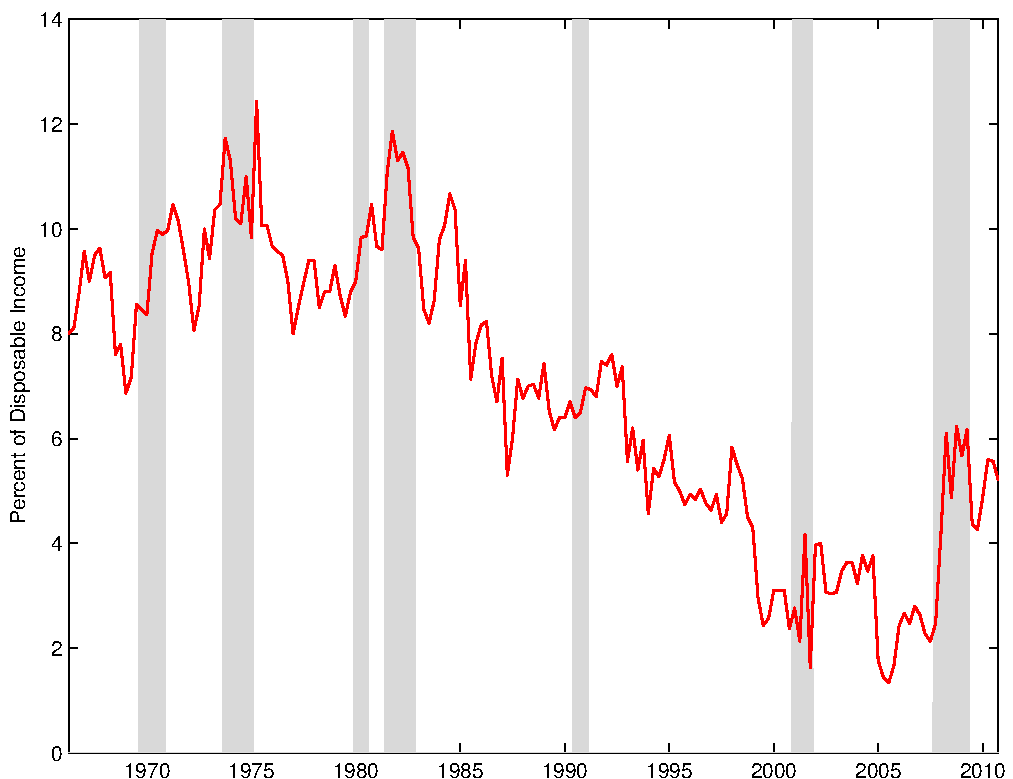
\includegraphics[height=3in,width=4.5in]{\econtexRoot/Figures/fPSR_slides.pdf}
    % \end{center}
  \end{figure}
\end{frame}

\begin{frame}\frametitle{\bf Theory}

  \begin{eqnarray}
    \valfn(\mRat_{t})&=&\underset{\{\cFunc_{t},\xFunc_{t}\}}{\max } ~~ \util(\cFunc_{t})+\Discount \Ex_{t}\left[ \valfn(\mRat_{t+1}) \notag
                         \right]   \label{eq:hetdecisionprobnashk}\\
    \notag &\text{s.t.}&\\
    \Rnorm_{t+1} & = & \zeta \mathbf{R}_{t+1}+(1-\zeta)\Rfree \notag \\
    \mRat_{t+1} & = & (\mRat_{t}-\xRat_{t}-\cRat_{t})\Rnorm_{t+1}+\tShkEmp_{t+1} \notag
  \end{eqnarray}

  \begin{itemize}
  \item Labor Income Uncertainty
    \begin{itemize}
    \item Unemployment Is Biggest Shock
    \item Lots of Micro Evidence that Precautionary Saving Is Big
    \item Basically, people facing greater $\sigma$:
      \begin{itemize}
      \item Don't buy a house/car  ($\xRat = 0$)
      \item Hold larger net worth
      \end{itemize}
    \end{itemize}
  \item Rate-Of-Return Uncertainty
    \begin{itemize}
    \item Theoretical effects on $C$ ambiguous
      \begin{itemize}
        \item For plausible parameter values, $\sigma \uparrow \Rightarrow C \uparrow$
      \end{itemize}
    \item Portfolio share in risky asset is reduced
    \end{itemize}
  \end{itemize}
\end{frame}

\begin{frame}\frametitle{\bf Literature on $C$ }

  \begin{itemize}
  \item \jemph{``Wealth Effects''}
    \begin{itemize}
    \item Modigliani, Klein, MPS model, ...
      \begin{itemize} \item $\sRat_{t} = -0.05 \mRat_{t}$ + other stuff
      \end{itemize}
    \end{itemize}
  \item \jemph{``Precautionary''}
    \begin{itemize}
    \item \cite{carroll:brookings}
      \begin{itemize}
      \item Saving rate rises in recessions
      \item $\Delta \log C_{t+1}$ strongly related to $\Ex_{t}(u_{t+1}-u_{t})$
      \end{itemize}
    \end{itemize}
  \item \jemph{``Credit Availability''}
    \begin{itemize}
    \item Secular Trend: \begin{itemize} \item \cite{parker_nberma_spendthrift}, \cite{dynanKohn07_indebtedness}, Muellbauer (many papers) \end{itemize}
    \item Cyclical Dynamics: \begin{itemize}
      \item \cite{glLiq}, \cite{gkLiq}, \cite{hall:slump} \end{itemize}
    \end{itemize}
  \end{itemize}


\end{frame}


\begin{frame}\frametitle{\textbf{Great Recession 2007--2009}}


  \begin{itemize}
  \item $\sRat$ rises by $\sim$4 pp
  \item \jemph{Bigger \&\ more persistent increase} than any postwar recession
  \item But all three indicators also move a lot:
    \begin{itemize}
    \item Credit conditions tighten
    \item Unemployment Expectations rise
    \item Wealth falls
    \end{itemize}
  \end{itemize}

\end{frame}



\begin{frame}
  \frametitle{\textbf{Personal Saving Rate 2007-- $\boldsymbol{\uparrow}$ %by 5 pp
    }}


  \begin{figure}
    % \begin{center}
    %   \vspace*{-4mm}
    %   \hspace*{-1.0cm}
    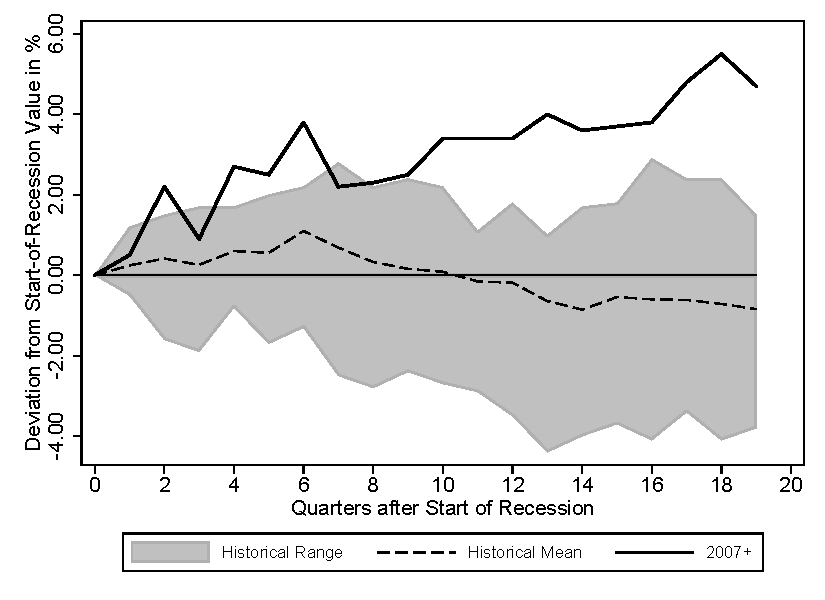
\includegraphics[height=3in,width=4.5in]{\econtexRoot/Figures/saving.pdf}
    % \end{center}
  \end{figure}
\end{frame}

\begin{verbatimwrite}{./PtnSlidesMovedToEnd-Wealth.tex}
  \begin{frame}
    \frametitle{\textbf{Household Wealth 2007--  $\boldsymbol{\downarrow}$ by 150\% of Income}}

    \begin{figure}
      % \begin{center}
      %   \vspace*{-4mm}
      %   \hspace*{-1.0cm}
      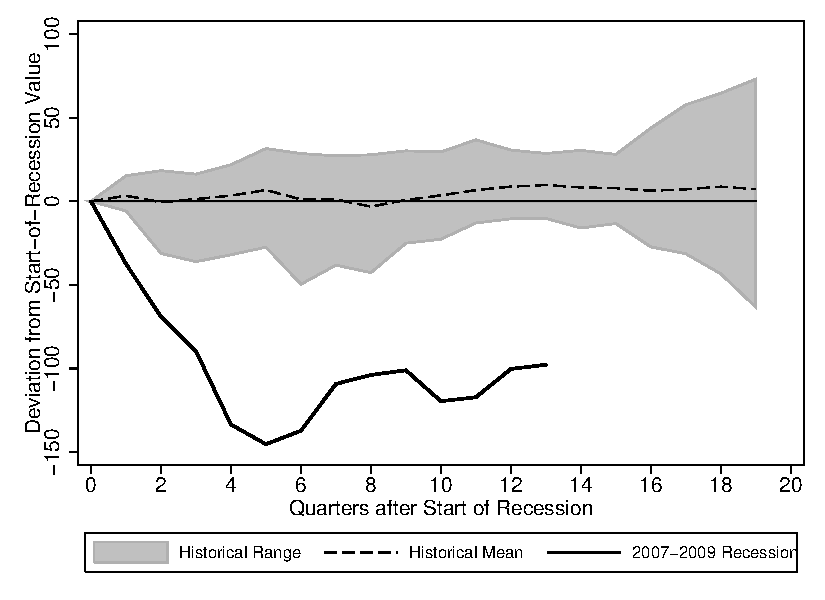
\includegraphics[height=3in,width=4.5in]{\econtexRoot/Figures/fWealth.pdf}
      % \end{center}
    \end{figure}
  \end{frame}
\end{verbatimwrite}


\ifPtn{ % Omit this slide from Princeton talk
}{
    \begin{frame}
    \frametitle{\textbf{Household Wealth 2007--  $\boldsymbol{\downarrow}$ by 150\% of Income}}

    \begin{figure}
      % \begin{center}
      %   \vspace*{-4mm}
      %   \hspace*{-1.0cm}
      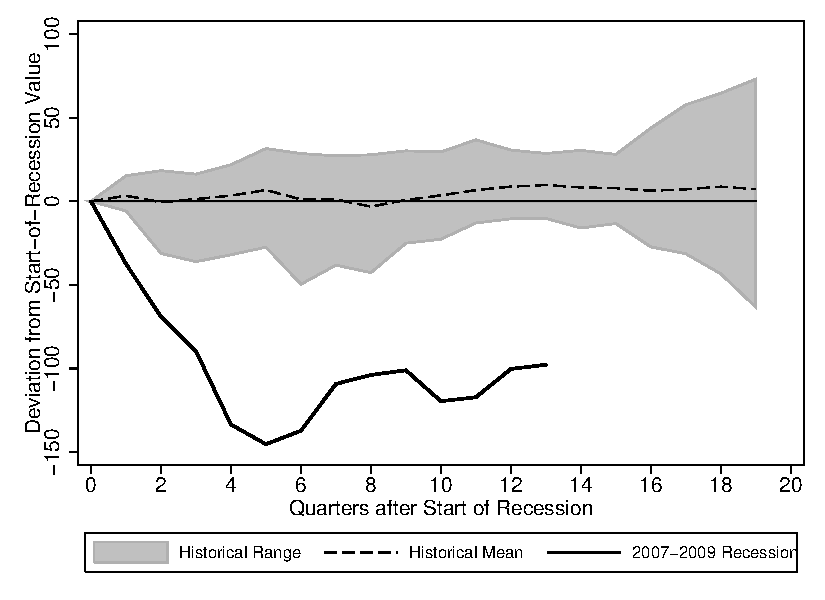
\includegraphics[height=3in,width=4.5in]{\econtexRoot/Figures/fWealth.pdf}
      % \end{center}
    \end{figure}
  \end{frame}

}


\begin{verbatimwrite}{./PtnSlidesMovedToEnd-URisk.tex}
  \begin{frame}
    \frametitle{\textbf{Sustained Expectations of \underline{Rising} Unemp Risk}}
    Thomson Reuters/University of Michigan $\Ex_{t}(u_{t+4}-u_{t})$

    \begin{figure}
      % \begin{center}
      %   \vspace*{-4mm}
      %   \hspace*{-1.0cm}
      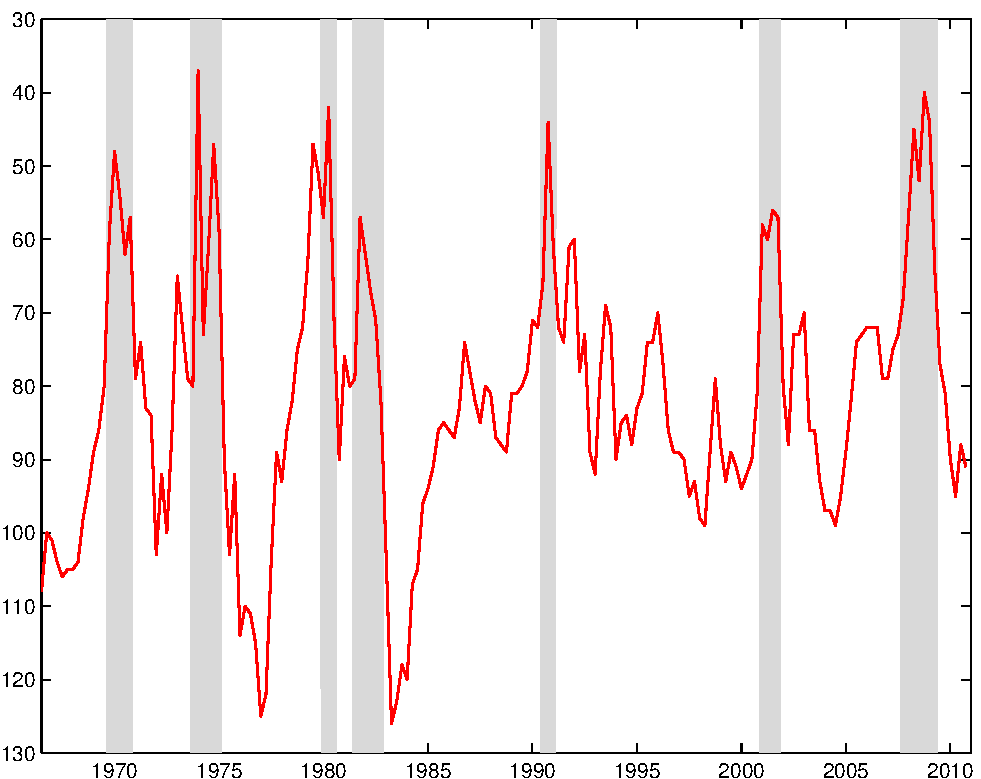
\includegraphics[height=2.8in,width=4.5in]{\econtexRoot/Figures/fUExp.pdf}
      % \end{center}
    \end{figure}
  \end{frame}
\end{verbatimwrite}


\ifPtn{ % Omit this slide from Princeton talk
}{
    \begin{frame}
    \frametitle{\textbf{Sustained Expectations of \underline{Rising} Unemp Risk}}
    Thomson Reuters/University of Michigan $\Ex_{t}(u_{t+4}-u_{t})$

    \begin{figure}
      % \begin{center}
      %   \vspace*{-4mm}
      %   \hspace*{-1.0cm}
      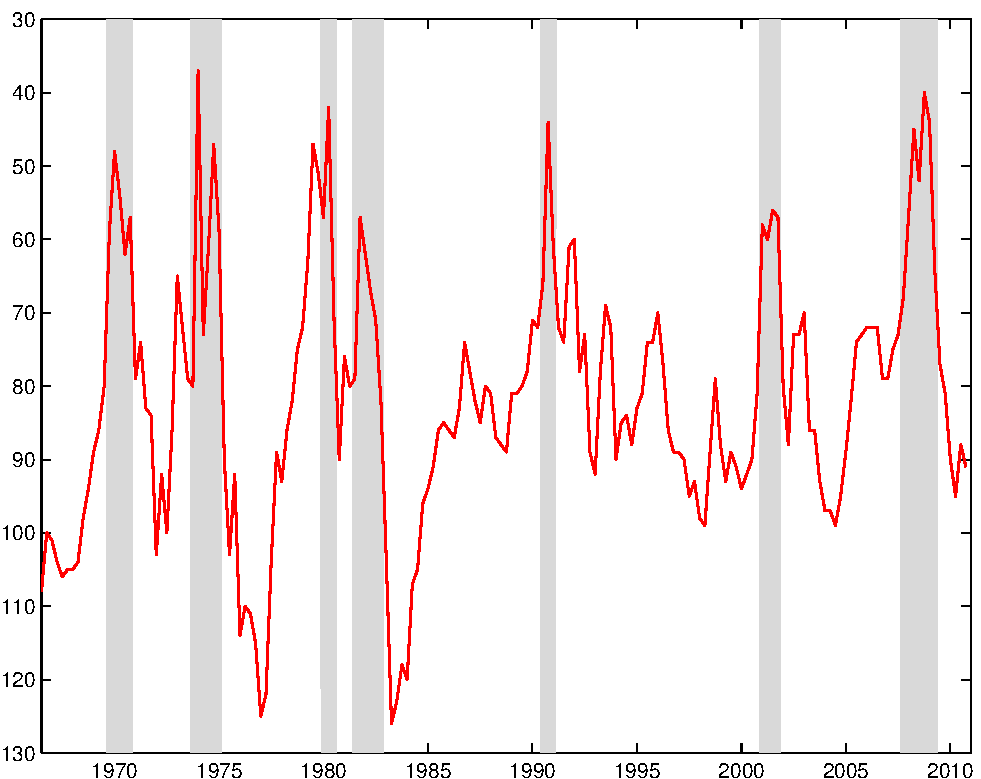
\includegraphics[height=2.8in,width=4.5in]{\econtexRoot/Figures/fUExp.pdf}
      % \end{center}
    \end{figure}
  \end{frame}

}


\begin{verbatimwrite}{./PtnSlidesMovedToEnd-CEA.tex}
  \begin{frame}
    \frametitle{\textbf{Tighter  HH Credit Supply (Based on Muellbauer)}}

    \begin{figure}
      % \begin{center}
      %   \vspace*{-4mm}
      %   \hspace*{-1.0cm}
      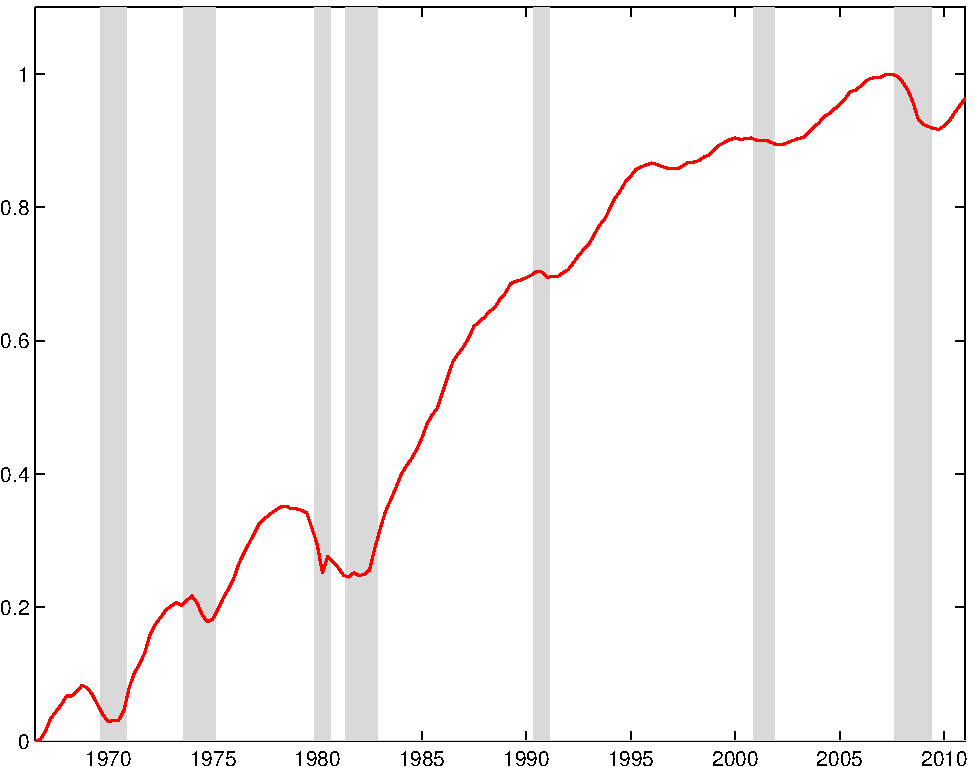
\includegraphics[height=3in,width=4.5in]{\econtexRoot/Figures/fCredit.pdf}
      % \end{center}
    \end{figure}
  \end{frame}
\end{verbatimwrite}

\ifPtn{ % Omit this slide from Princeton talk
}{
  \input {./PtnSlidesMovedToEnd-Credit.tex}
}



\ifSFFed{}{
  \begin{frame}\frametitle{\textbf{Our Contributions}}

    \begin{itemize}
    \item \jemph{Theory}
      \begin{itemize}
      \item Simple model with transparent role for all 3 channels
      \item Qualitative implications of the model
        \begin{itemize} \item ``Overshooting'' $\Rightarrow$ possible role for fiscal policy
        \end{itemize}
      \end{itemize}
    \item \jemph{Evidence}
      \begin{itemize}
      \item Quantify the 3 channels
      \item Two estimated models of $\sRat$
        \begin{itemize}
        \item \jemph{Reduced-form}---OLS
        \item \jemph{Structural}---Nonlinear least squares
        \end{itemize}
      \end{itemize}
    \item \jemph{Conclusions}
      \begin{itemize}
      \item {\it Secular} decline in $\sRat$ is almost all from credit $\uparrow$
      \item {\it Cyclical} movement in $\sRat$ is mostly from $w$ and $\mho$
      \item Any big cyclical effect of credit {\it runs through} effects on $w$, $\mho$
      \end{itemize}
    \end{itemize}

  \end{frame}

  \ifPtn{}{
    \begin{frame}
      \frametitle{\textbf{Why Do We Care?}}

      \begin{itemize}
        % \item Quantify impact of key determinants on \jemph{$\sRat$}
      \item \jemph{\it Quantify} role of \jemph{credit, wealth and uncertainty}
      \item Useful for in-sample and out-of-sample analysis
      \item \jemph{Strength of recovery}/dynamics of GDP
        % \item Time variation in \jemph{target wealth}
        % \item Use larger-scale models (not univariate)
      \end{itemize}

    \end{frame}
  }



  \begin{frame}
    \frametitle{\textbf{Theory \`a la \cite{ctDiscrete}}}

    \begin{itemize}
    \item CRRA utility, labor supply $\ell$, agg wage $\Wage$, emp status $\xi$:
      \begin{eqnarray*}
        \valfn(\mLev_{t})&=&\underset{\cLev_{t}}{\max } ~~
                             \util(\cLev_{t})+\Discount \Ex_{t}\begin{itemize}g[ \valfn(\mLev_{t+1})
                               \big]  \label{eq:hetdecisionprobnashk}\\
                               \notag &\text{s.t.}&\\
                               \mLev_{t+1} & = & (\mLev_{t}-\cLev_{t})\Rfree +\labor_{t+1}\Wage_{t+1}\empState_{t+1}  \label{eq:DBC}
                             \end{eqnarray*}
                                                 \item $\empState_{t+1} \in \{\empState^{u},\empState^{e}\}$ where $\empState^{u} < \empState^{e}$
                                                 \item $\labor$ and $\Wage$ grow at constant rate
                                                   % \begin{itemize}
                                                   % \item CT model: $\{\empState^{u},\empState^{e}\}=\{0,1\}$
                                                   % \item Our model: wage-tax-financed UI system so $\empState^{u} > 0$
                                                   % \end{itemize}
                                                 \item Tractability: unemployment shocks are \jemph{permanent}
                                                 \begin{itemize}
                                                 \item If $\empState_{t}=\empState^{u}$ then $\empState_{t+1}=\empState^{u}$
                                                 \end{itemize}
                                                 \item \jemph{Target wealth $\mTarg$} exists and is stable:
                                                 \begin{itemize}
                                                 \item Consumption chosen so that $\mRat_t\rightarrow \mTarg$
                                                 \end{itemize}
                                                 \end{itemize}

                                               \end{frame}



                                               \begin{verbatimwrite}{./PtnSlidesMovedToEnd-ConsFunc.tex}
                                                 \begin{frame}
                                                   \frametitle{\textbf{Consumption Function}}

                                                   \begin{figure}
                                                     % \begin{center}
                                                     %   \vspace*{-4mm}
                                                     %   \hspace*{-1.0cm}
                                                     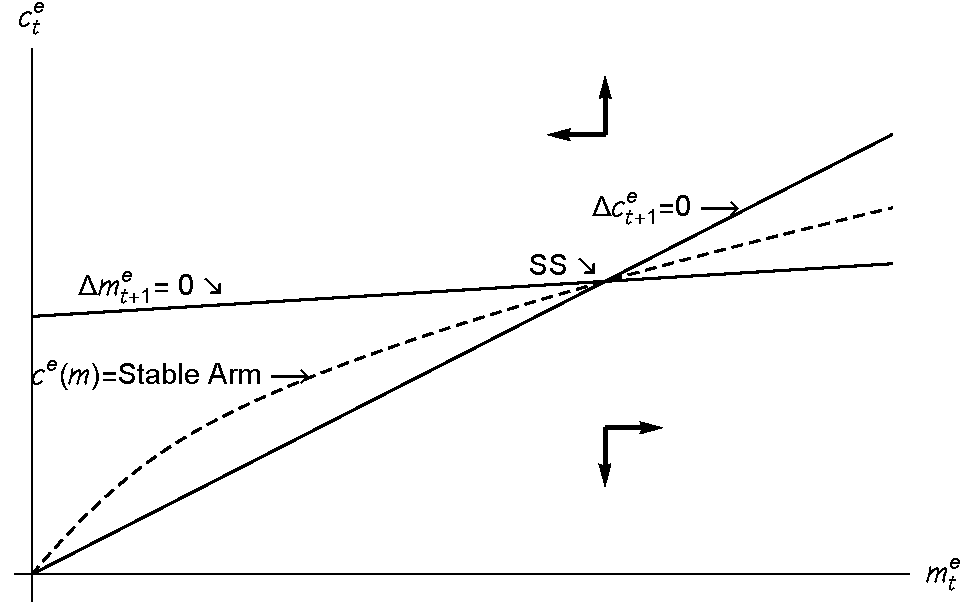
\includegraphics[height=3in,width=4.5in]{\econtexRoot/Figures/TractableBufferStockPhaseDiag.pdf}
                                                     % \end{center}
                                                   \end{figure}
                                                 \end{frame}
                                               \end{verbatimwrite}
                                               \ifPtn{}{
                                                 \input \econtexRoot/Slides/PtnSlidesMovedToEnd-ConsFunc.tex
                                               }



                                               \begin{frame}
                                                 \frametitle{\textbf{Target Wealth} $\mTarg$}

                                                 Closed-form solution for target wealth depends on unemployment risk $\urate$ and generosity of unemployment insurance $\empState^{u}$:
                                                 $$
                                                 \jemph{\mTarg=f(\mathop{\urate}_{(+)},\mathop{\empState^{u}}_{(-)},\text{preferences}, \dots) \label{mTargetNonlin}}
                                                 $$
                                                 % where $\urate$ is unemployment risk.

                                                 % Why does target wealth decline in $\empState^{u}$?
                                                 % \begin{itemize}
                                                 % \item $\empState^{u} \uparrow$ relaxes `Natural Borrowing Constraint' (NBC)
                                                 % \item NBC: `never end with $\aRat_{t}$ so low that $\cRat_{t+1} = 0$ is possible'
                                                 % \item PDV of unemployment benefits is $\empState^{u}/(\Rnorm-1)$
                                                 % \item So NBC says $a_{t} > -\empState^{u}/(\Rnorm-1)$
                                                 % \end{itemize}
                                                 % 
                                                 % We {\it could} add a tighter, `artificial' borrowing constraint
                                                 % \begin{itemize}
                                                 % \item But tightening natural borrowing constraint is just like tightening artificial one
                                                 % \item Adds complexity to the model without adding insight
                                                 % \end{itemize}
                                                 % 
                                                 % $\Rightarrow$ we assume our measure of credit conditions identifies NBC
                                                 % \end{comment}

                                               \end{frame}

                                               \begin{frame}\frametitle{\textbf{Consumption After a Wealth Shock}}
                                                 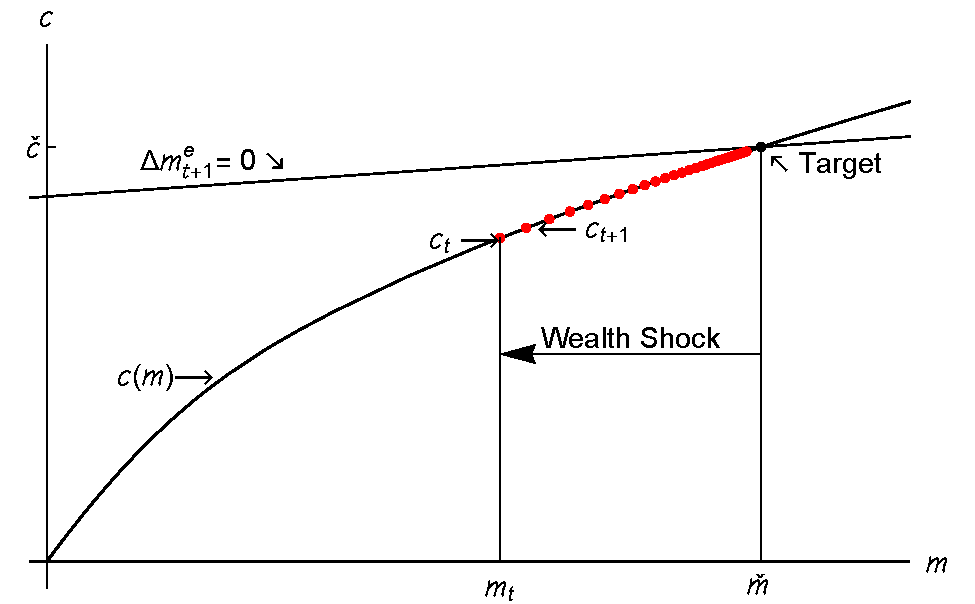
\includegraphics[width=4in]{\econtexRoot/Figures/WealthShock.pdf}
                                               \end{frame}

                                               \begin{frame}\frametitle{\textbf{Permanent Rise in $\urate$}}

                                                 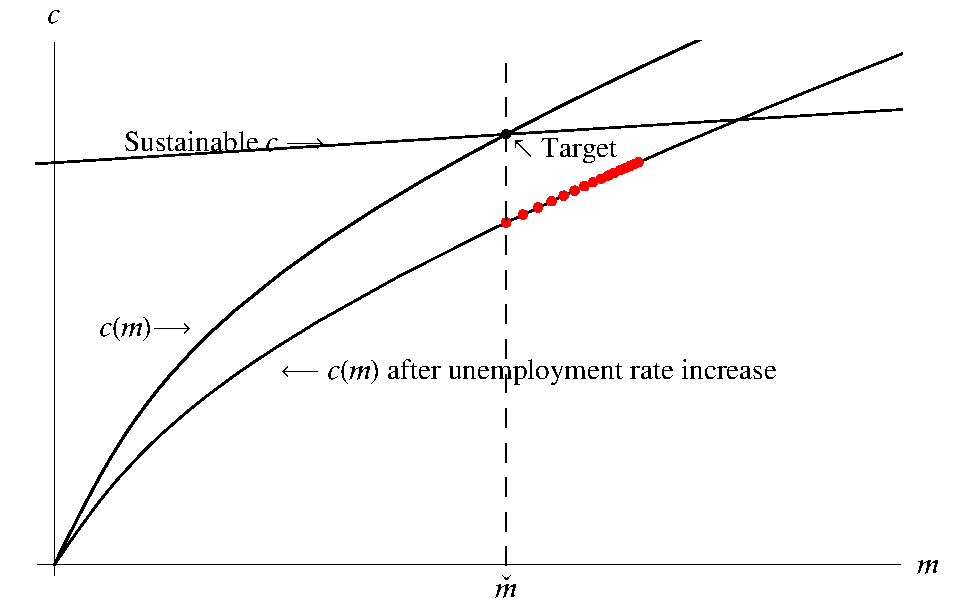
\includegraphics[width=4in]{\econtexRoot/Figures/cBeforeAndAfteruRise.pdf}

                                               \end{frame}

                                             }

                                             \begin{frame}\frametitle{\textbf{Saving Rate After a Permanent Rise in $\urate$}}

                                               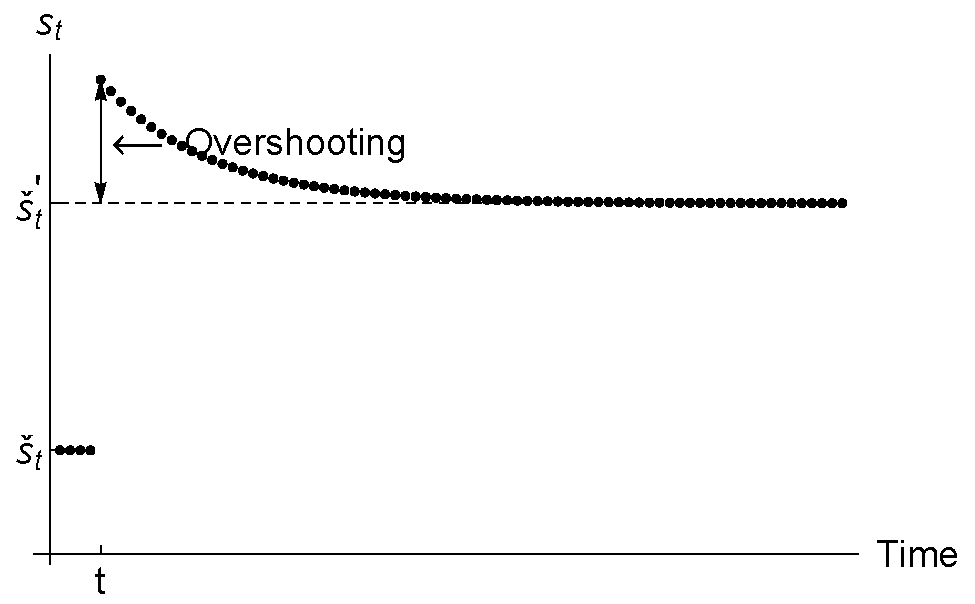
\includegraphics[width=4in]{\econtexRoot/Figures/savRateAfterMhoRisePlot.pdf}

                                             \end{frame}

                                             \begin{verbatimwrite}{./PtnSlidesMovedToEnd-Overshooting.tex}
                                               \begin{frame}\frametitle{\bf Overshooting and Fiscal Policy}

                                                 DSGE models:
                                                 \begin{itemize}
                                                 \item Frictions, frictions everywhere; but missing here
                                                 \item If $\Delta \cRat$ imposes `external' costs
                                                   \begin{itemize}
                                                   \item Sticky prices/wages
                                                   \item Capital (or Investment) adjustment costs
                                                   \item Other reasons for `pecuniary externalities'
                                                   \end{itemize}
                                                 \item $\Rightarrow$ `stimulus' payments, fiscal policy may reduce cost of cycle
                                                 \item Justification for `automatic stabilizers'?
                                                 \end{itemize}

                                               \end{frame}
                                             \end{verbatimwrite}

                                             \ifPtn{}{
                                               \input \econtexRoot/Slides/PtnSlidesMovedToEnd-Overshooting.tex
                                             }




                                             \begin{frame}
                                               \frametitle{\textbf{Credit Easing/Financial Innovation \& Deregulation}}

                                               \begin{figure}
                                                 % \begin{center}
                                                 %   \vspace*{-4mm}
                                                 %   \hspace*{-1.0cm}
                                                 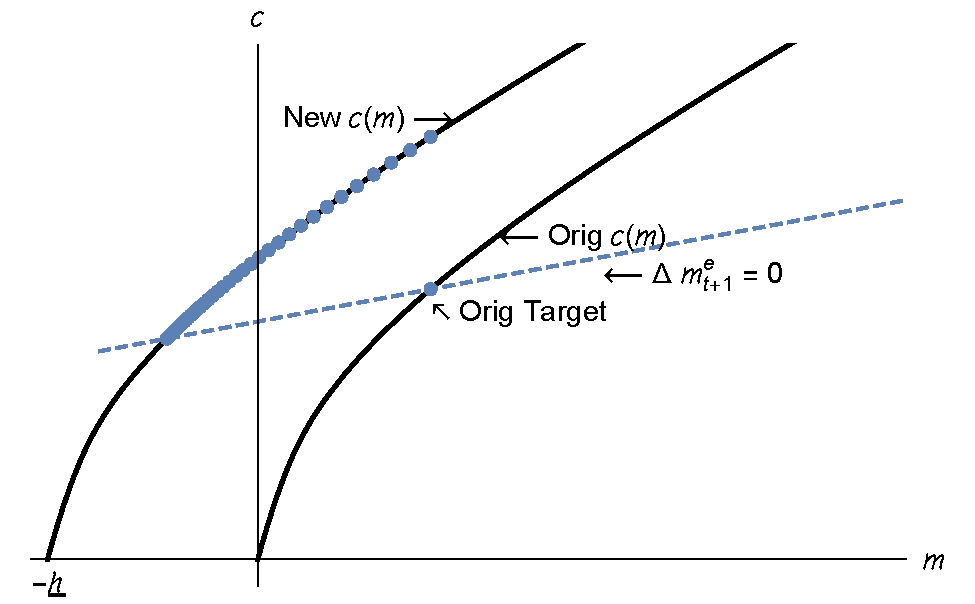
\includegraphics[width=3.5in]{\econtexRoot/Figures/PhaseDiagramDebtLimRisePlot.pdf}
                                                 % \end{center}
                                               \end{figure}

                                               \jemph{$\mTarg$ is close to linear in credit conditions}

                                             \end{frame}

                                             \ifPtn{}{
                                               \begin{frame}
                                                 \frametitle{\textbf{Data \& Sources}}

                                                 \begin{itemize}
                                                 \item Quarterly 1966Q2--2011Q1
                                                 \item \jemph{Saving rate:} BEA NIPA
                                                 \item \jemph{Net worth:}  Flow of Funds Accounts, Fed
                                                   \begin{itemize}
                                                   \item (Model $m$ corresponds to 1 + ratio of Net worth to disposable income)
                                                   \end{itemize}
                                                 \item \jemph{Credit conditions:} ``Credit Easing Accumulated,'' CEA
                                                   \bi \item Senior Loan Officer Opinion Survey (SLOOS), Fed
                                                 \item {\footnotesize Banks' \jemph{willingness} to provide consumer installment loans}
                                                 \end{itemize}
                                               \item \jemph{Unemployment risk:} using Thomson Reuters/UMichigan unemployment expectations
                                               \end{itemize}

                                             \end{frame}
                                           }

                                           \begin{frame}
                                             \frametitle{\textbf{Net Worth (Ratio to Quarterly Disp Income)}}

                                             \begin{figure}
                                               % \begin{center}
                                               %   \vspace*{-4mm}
                                               %   \hspace*{-1.0cm}
                                               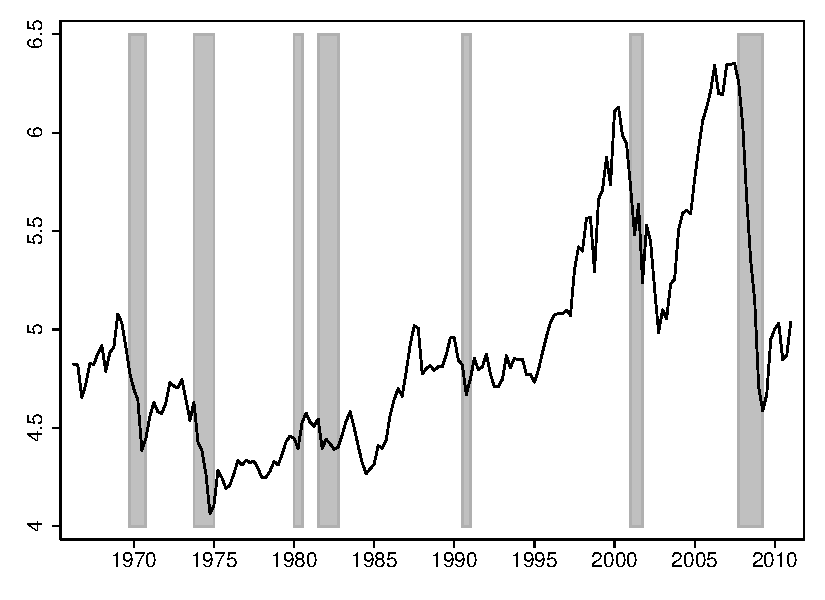
\includegraphics[height=3in,width=4.5in]{\econtexRoot/Figures/fWyRat.pdf}
                                               % \end{center}
                                             \end{figure}

                                           \end{frame}

                                           \begin{frame}
                                             \frametitle{\textbf{Credit Easing Accumulated (CEA) (\`a la Muellbauer)}}
                                             Accumulated responses, weighted with debt--income ratio, to: \\
                                             \footnotesize{``Please indicate your \jemph{bank's willingness to make consumer installment loans} now as opposed to three months ago.''}

                                             \begin{figure}
                                               % \begin{center}
                                               %   \vspace*{-4mm}
                                               %   \hspace*{-1.0cm}
                                               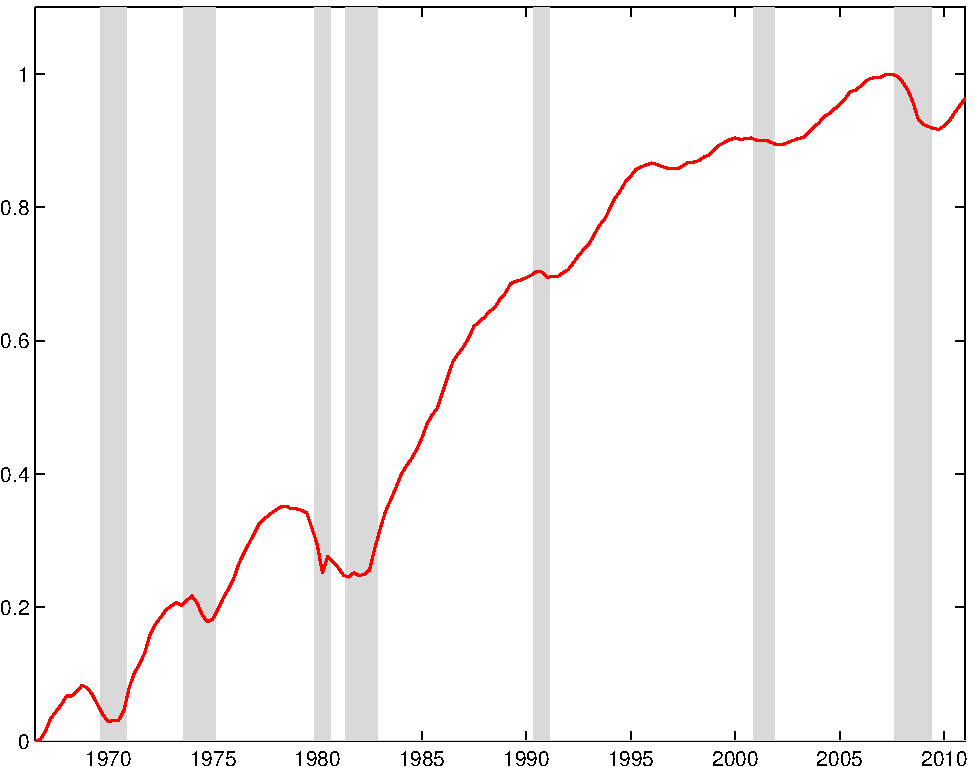
\includegraphics[height=2.5in,width=4.5in]{\econtexRoot/Figures/fCredit.pdf}
                                               % \end{center}
                                             \end{figure}

                                           \end{frame}


                                           \begin{frame}
                                             \frametitle{\textbf{$\urate_t$ Implied by Michigan U Expectations}}
                                             \ifSFFed{}{
                                               \bi \footnotesize
                                             \item Regress: $\Delta_4 u_{t+4}=\alpha_0+\alpha_1 UExp_t$
                                             \item \jemph{U risk: $\urate_t=u_t+\Delta_4 \hat{u}_{t+4}$}
                                             \item $\Delta_4 u_{t+4}\equiv u_{t+4}-u_t,\qquad \Delta_4 \hat{u}_{t+4}\equiv{} \text{fitted values}$
                                             \item $\mho_t$ tracks \jemph{but precedes} actual U
                                             \end{itemize}
                                           }
                                           {\scriptsize $UExp$: ``How about people out of work during the coming 12 months---do you think that there will be more unemployment than now, about the same, or less?''}
                                           \begin{figure}
                                             % \begin{center}
                                             %   \vspace*{-4mm}
                                             %   \hspace*{-1.0cm}
                                             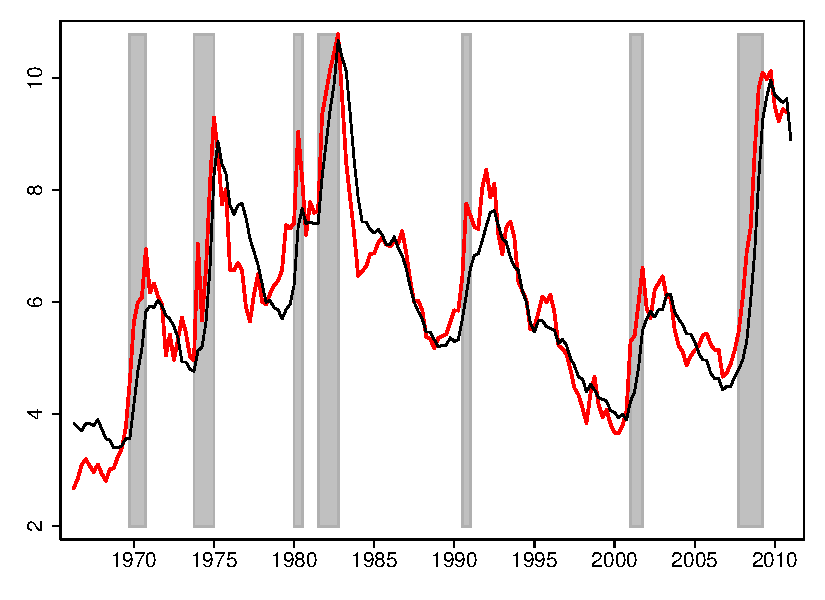
\includegraphics[height=2.35in,width=3.5in]{\econtexRoot/Figures/mhoUnem.pdf}
                                             % \end{center}
                                           \end{figure}

                                         \end{frame}


                                         \begin{frame}
                                           \frametitle{\textbf{Reduced-Form Regressions}}

                                           {\small\jemph{$s_t=\gamma_0+\gamma_m m_t +\gamma_{\CEA} \CEA_t+\gamma_{Eu}\Ex_t u_{t+4}+\gamma_t\,t+\gamma_{uC} (\Ex_t u_{t+4}\times\CEA_t)+\varepsilon_t $}}

                                           \input \econtexRoot/Tables/tOLS_prelim_time_slides.tex

                                         \end{frame}

                                         \ifSFFed{}{
                                           \begin{frame}
                                             \frametitle{\textbf{Fit: Baseline vs Time Trend}}

                                             \begin{figure}
                                               % \begin{center}
                                               %   \vspace*{-4mm}
                                               %   \hspace*{-1.0cm}
                                               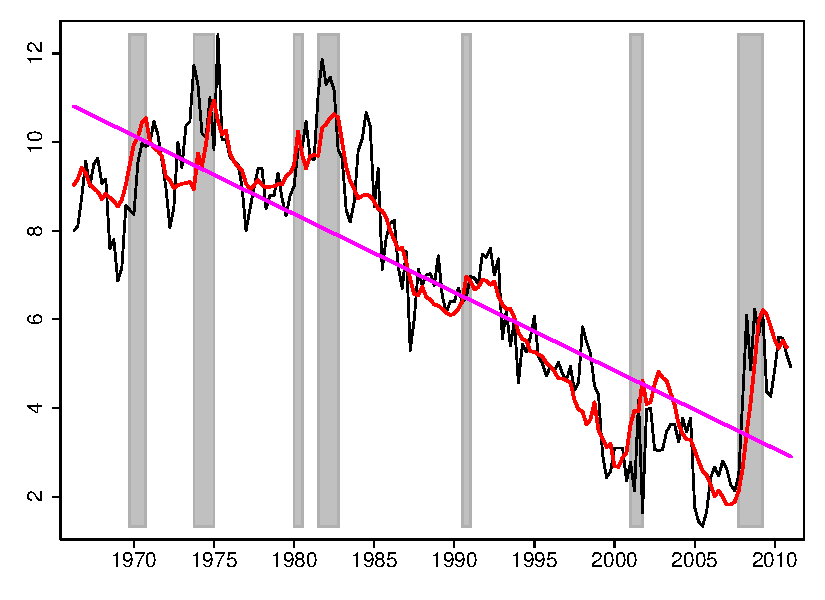
\includegraphics[height=3in,width=4.5in]{\econtexRoot/Figures/fOLS_fit_time_compare_slides.pdf}
                                               % \end{center}
                                             \end{figure}
                                           \end{frame}


                                           \begin{frame}
                                             {\small $s_t=\gamma_1+\gamma_m m_t +\gamma_{\CEA}\CEA_t+\gamma_{Eu}\Ex_t u_{t+4}+\gamma'X_t+\varepsilon_t $}
                                             \input \econtexRoot/Tables/tOLS02_slides.tex

                                           \end{frame}
                                         }{}

                                         \ifSFFed{}{
                                           \begin{frame}
                                             \frametitle{\textbf{Fit: Baseline vs Post-1980}}

                                             \begin{figure}
                                               % \begin{center}
                                               %   \vspace*{-4mm}
                                               %   \hspace*{-1.0cm}
                                               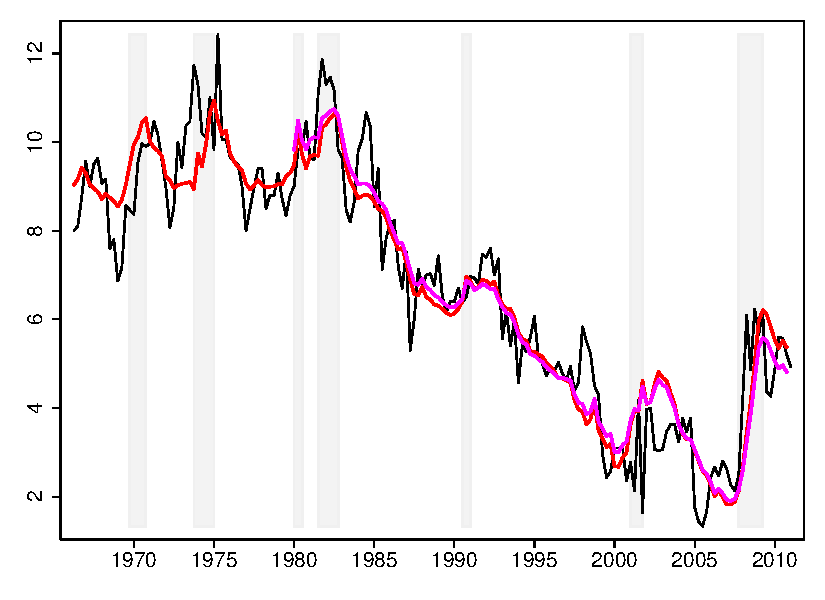
\includegraphics[height=3in,width=4.5in]{\econtexRoot/Figures/fPost80_slides.pdf}
                                               % \end{center}
                                             \end{figure}
                                           \end{frame}


                                           \begin{frame}
                                             \frametitle{\textbf{Fit: Baseline vs Full Controls}}

                                             \begin{figure}
                                               % \begin{center}
                                               %   \vspace*{-4mm}
                                               %   \hspace*{-1.0cm}
                                               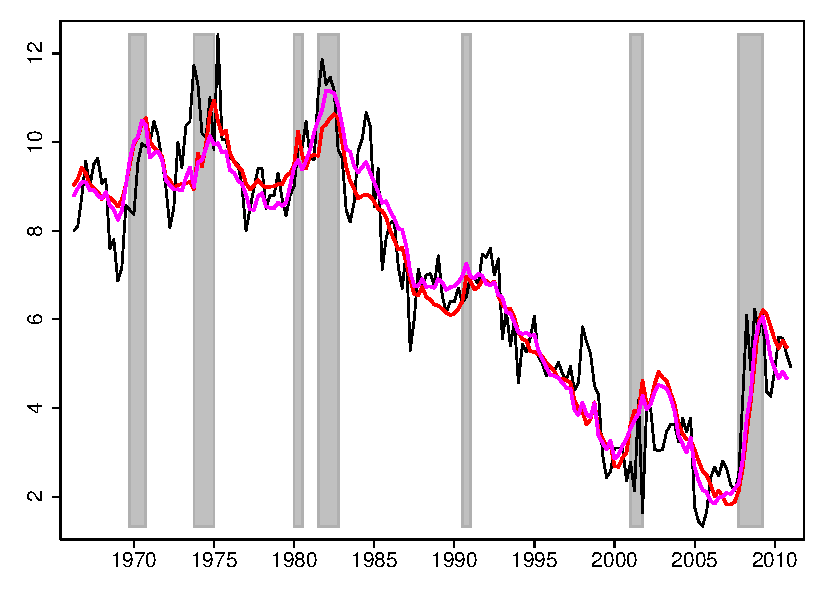
\includegraphics[height=3in,width=4.5in]{\econtexRoot/Figures/fFullControls_slides.pdf}
                                               % \end{center}
                                             \end{figure}
                                           \end{frame}


                                           \ifPtn{}{

                                             \begin{frame}
                                               \frametitle{\textbf{Reduced-Form Regressions---Summary}}
                                               The three factors explain saving well:
                                               \begin{enumerate}
                                               \item Credit conditions
                                               \item Wealth
                                               \item Unemployment risk
                                               \end{enumerate}

                                             \end{frame}
                                           }

                                         }

                                         \ifSFFed{}{
                                           \begin{frame}
                                             \frametitle{\textbf{Structural Estimation---Nonlinear Least Squares }}
                                             Minimize distance between model-implied \jemph{$s_t^{\text{theor}}$} and actual \jemph{$s_{t}^{\text{meas}}$}:

                                             $$
                                             \hat{\Theta}=\argmin
                                             \sum_{t=1}^T\bigg(s_{t}^{\text{meas}}-s_t^{\text{theor}}\Big(\Theta;
                                             \mRat_t-\check{\mRat}\big(\bar{m}(\CEA_t),\mho(\Ex_tu_{t+4})\big)\Big)\bigg)^2,
                                             $$
                                             where
                                             \begin{itemize}
                                             \item $\Theta=\{\Discount,\bar{\theta}_m,\theta_\CEA,\bar{\theta}_\mho,\theta_u\}$
                                             \item $\bar{\mRat}_t=\bar{\theta}_\mRat+\theta_\CEA \CEA_t$
                                             \item $\mho_t=\bar{\theta}_\mho+\theta_u \Ex_tu_{t+4}$
                                             \item $\Discount$: discount factor
                                             \end{itemize}

                                           \end{frame}
                                         }


                                         \ifPtn{}{
                                           \begin{frame}
                                             \frametitle{\textbf{Structural Estimation---Asymptotics }}

                                             \begin{block}{Delta Method}
                                               $$
                                               T^{1/2}(\hat{\Theta}-\Theta)\rightarrow_d \mathcal{N}(0, D^{-1}ED'^{-1}),
                                               $$
                                               where
                                               \begin{itemize}
                                               \item $D=\Ex\frac{\partial q_t(\Theta)}{\partial \Theta'}$
                                               \item $E=\var\big(q_t(\Theta)\big)$
                                               \item Scores $q_t(\Theta)=\big(s_{t}^{\text{meas}}-s_t^{\text{theor}}(\Theta)\big)\frac{\partial s_t^{\text{theor}}(\Theta)}{\partial \Theta'}$
                                               \end{itemize}
                                             \end{block}

                                           \end{frame}


                                           \begin{frame}
                                             \frametitle{\textbf{Structural Estimates }}
                                             \input \econtexRoot/Tables/tStructEst_slides.tex
                                           \end{frame}

                                           \begin{frame}\frametitle{\large\textbf{Estimated Credit Effect on $\bar{m}_t$ (Frac of DI)}}
                                             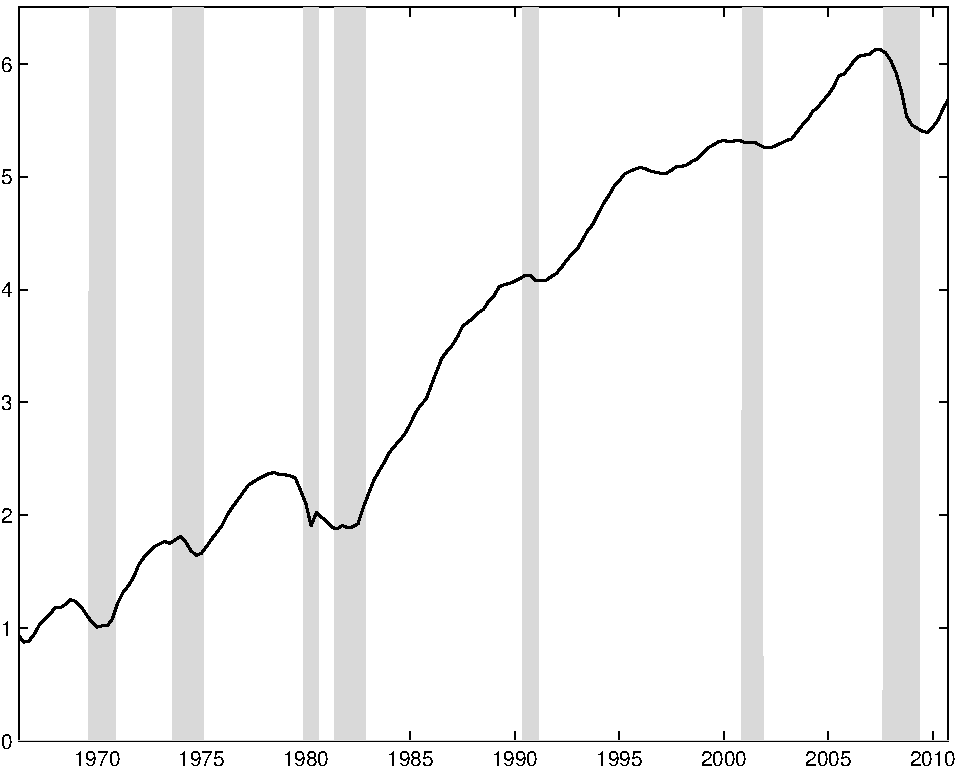
\includegraphics[width=4in]{\econtexRoot/Figures/fCEA_est.pdf}
                                           \end{frame}

                                         }


                                         \ifPtn{}{
                                           \begin{frame}\frametitle{\textbf{Estimated Unemployment Risk $\mho_t$}}
                                             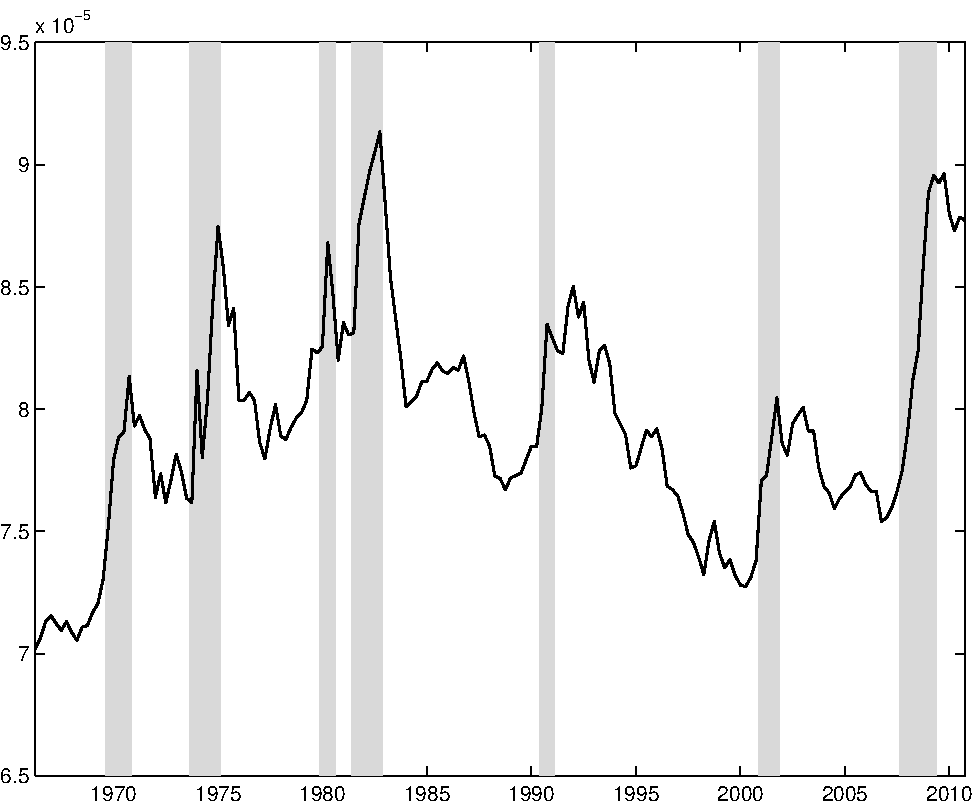
\includegraphics[width=4in]{\econtexRoot/Figures/fMho_est.pdf}
                                           \end{frame}
                                         }



                                         % \begin{frame}\frametitle{\textbf{Estimated Consumption Function}}
                                         %   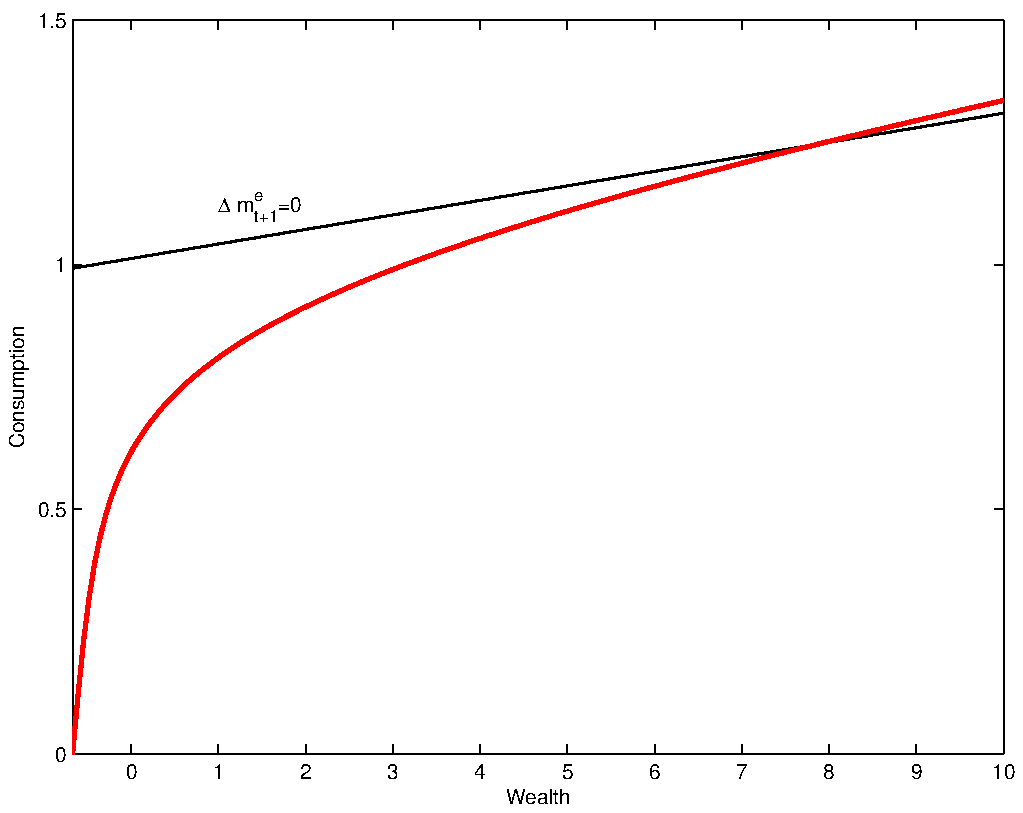
\includegraphics[width=4in]{\econtexRoot/Figures/fEstCfunction.pdf}
                                         % \end{frame}

                                         \ifSFFed{}{
                                           \begin{frame}\frametitle{\textbf{Fit of the Structural Model}}
                                             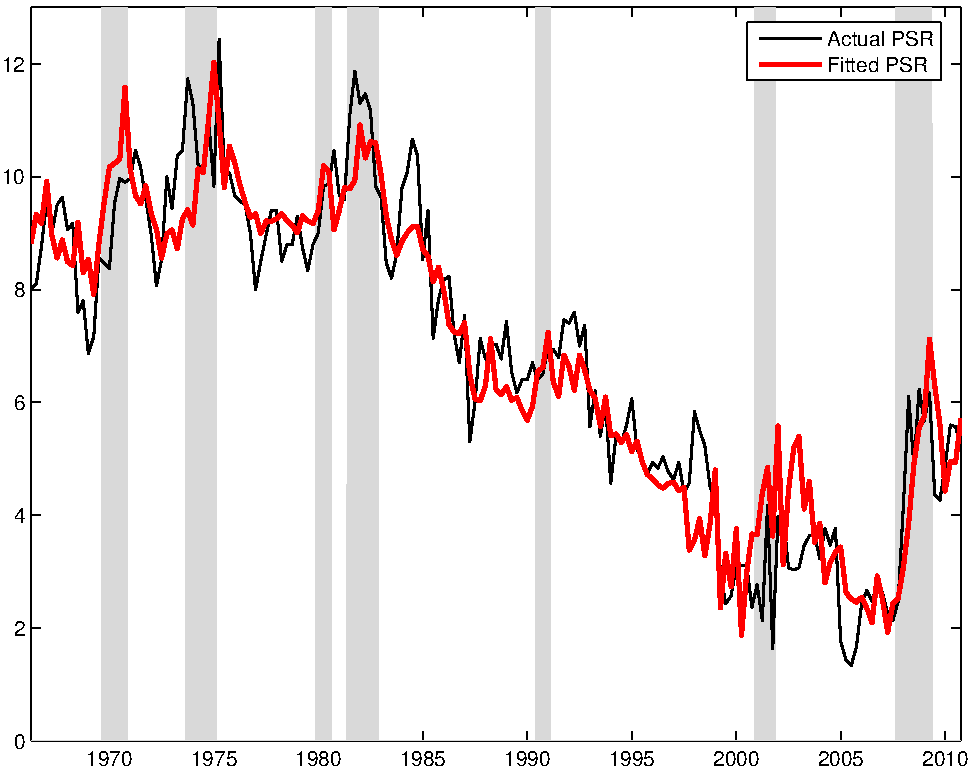
\includegraphics[width=4in]{\econtexRoot/Figures/fPSR_StructFit_slides.pdf}
                                           \end{frame}

                                           \begin{frame}\frametitle{\textbf{Decomposition of Fitted PSR}}
                                             Fix $\mho_t$ and $\CEA_t$ at their sample means, back out the implied $\sRat_t$\\
                                             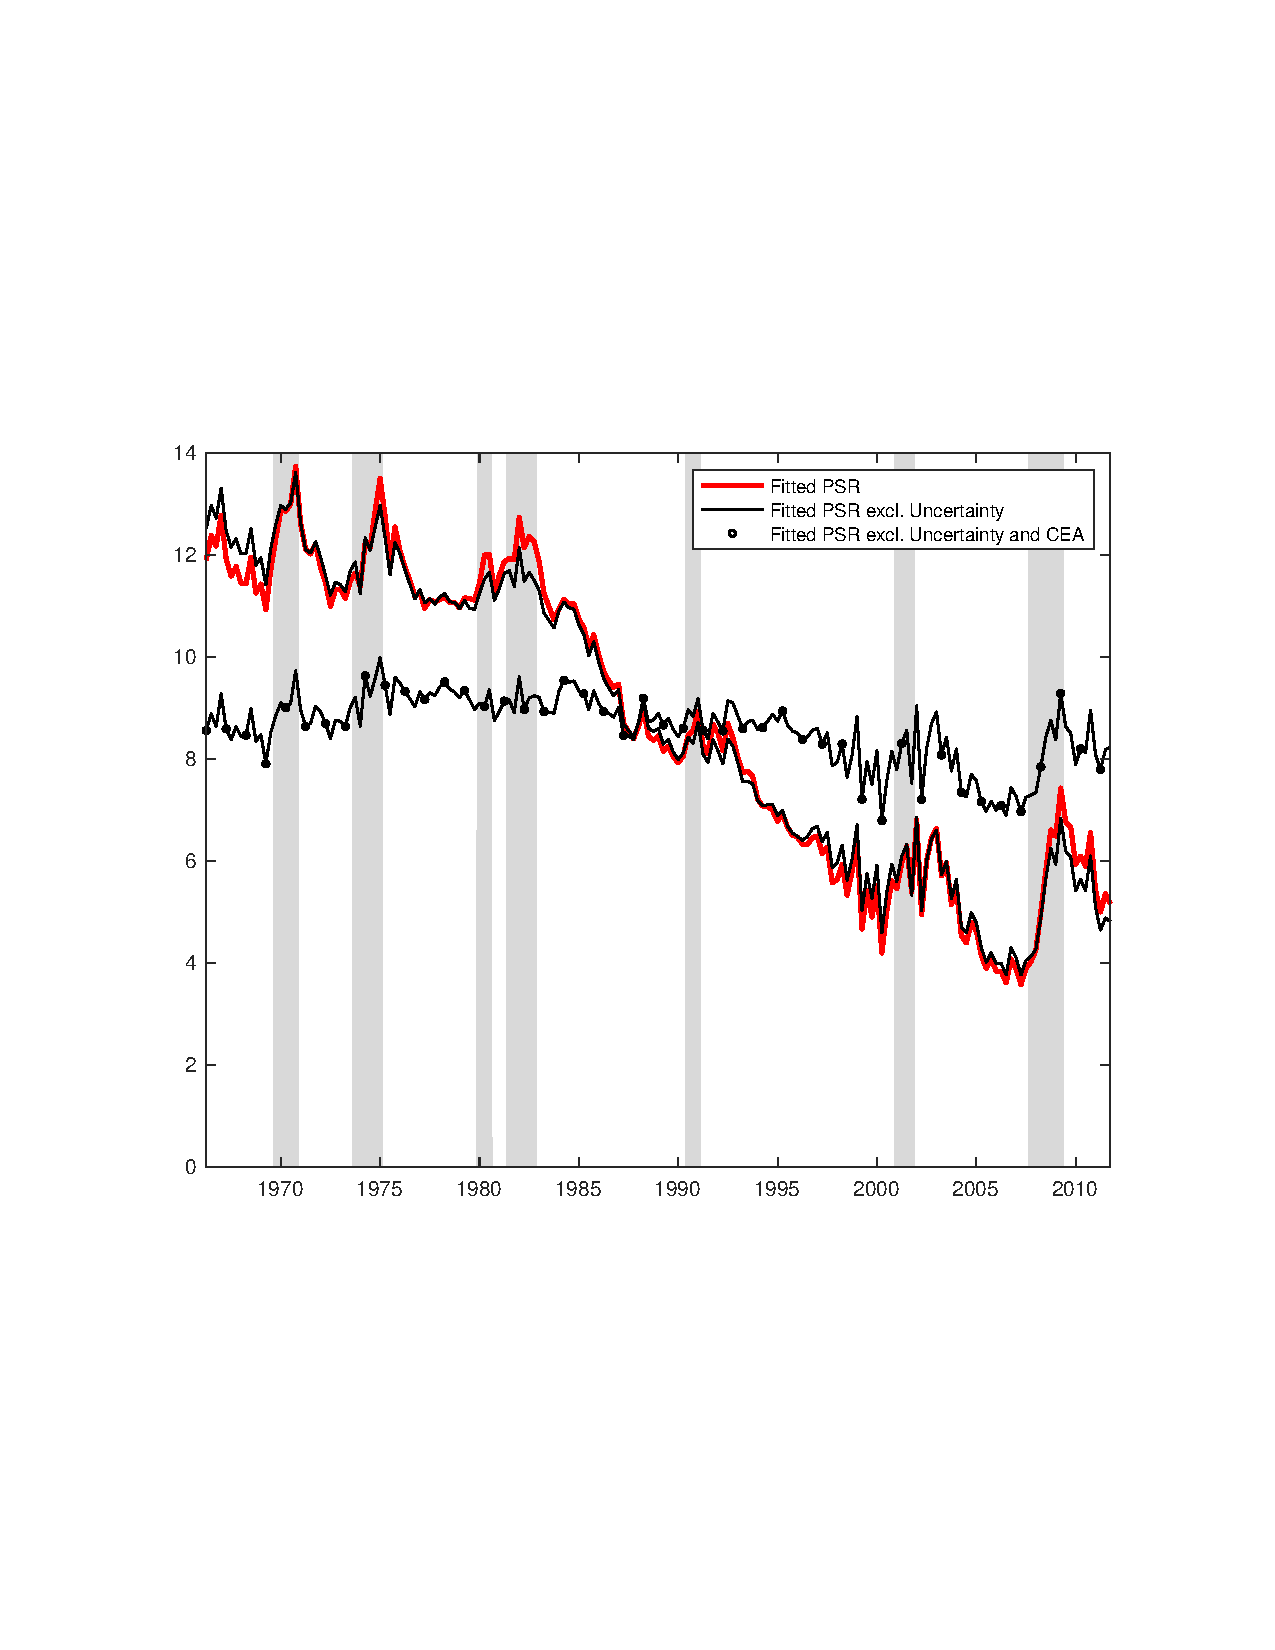
\includegraphics[width=4in]{\econtexRoot/Figures/fPSR_StructDecomp.pdf}
                                           \end{frame}



                                           \begin{frame}\frametitle{\textbf{Fit: Structural Model vs Reduced-Form}}
                                             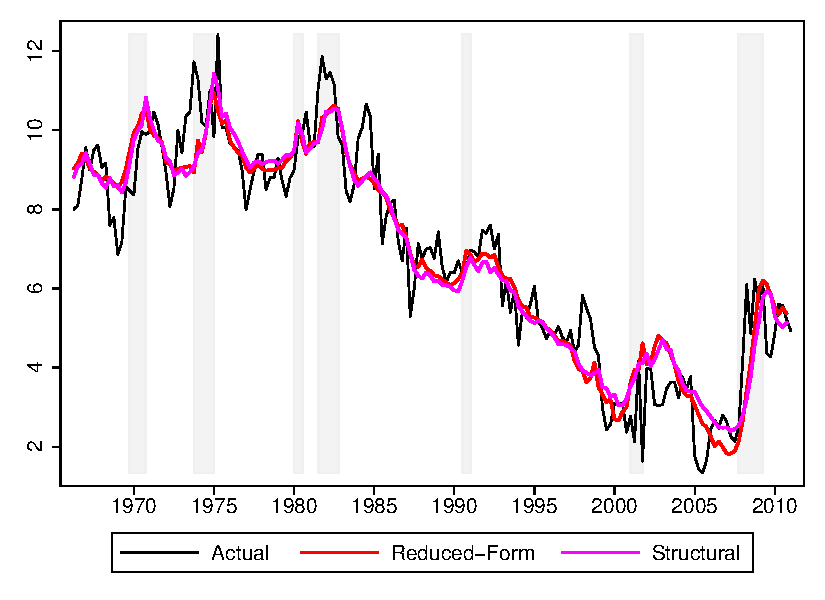
\includegraphics[width=4in]{\econtexRoot/Figures/fOLS_fit_redStruct_compare.pdf}
                                           \end{frame}

                                           \begin{verbatimwrite}{./PtnSlidesMovedToEnd-ReducedForm.tex}
                                             \begin{frame}
                                               \frametitle{\textbf{Reduced-Form Regressions on Model Data}}

                                               {\small\jemph{$s_t^{\text{theor}}=\gamma_0+\gamma_m m_t +\gamma_{\CEA} \CEA_t+\gamma_{Eu}\Ex_t u_{t+4}+\gamma_t\,t+\gamma_{uC} (\Ex_t u_{t+4}\times\CEA_t)+\varepsilon_t $}}

                                               \input \econtexRoot/Tables/tOLS_prelim_time_model_slides.tex

                                             \end{frame}


                                             \begin{frame}
                                               \frametitle{\textbf{Reduced-Form Regressions on Actual Data}}

                                               {\small\jemph{$s_t^{\text{meas}}=\gamma_0+\gamma_m m_t +\gamma_{\CEA} \CEA_t+\gamma_{Eu}\Ex_t u_{t+4}+\gamma_t\,t+\gamma_{uC} (\Ex_t u_{t+4}\times\CEA_t)+\varepsilon_t $}}

                                               \input \econtexRoot/Tables/tOLS_prelim_time_slides.tex

                                             \end{frame}


                                           \end{verbatimwrite}


                                           \input \econtexRoot/Slides/PtnSlidesMovedToEnd-ReducedForm.tex

                                           \begin{frame}
                                             \frametitle{\textbf{Structural Estimation---Summary}}

                                             \begin{itemize}
                                             \item Model fits well\dots
                                             \item \dots almost as well as reduced form\\ (Mincer--Zarnowitz puts weight 0.45 on structural model)
                                             \item Substantial role for \jemph{time-varying precautionary saving}
                                             \item \CEA\ matters for low frequency,\\ wealth for business-cycle frequency
                                             \end{itemize}

                                           \end{frame}

                                         }


                                         \ifSFFed{}{
                                           \begin{frame}
                                             \frametitle{\textbf{PSR Forecasts---In Sample}}

                                             \begin{block}{Great Recession 2007--2010}
                                               \input \econtexRoot/Tables/tPred_structRF.tex
                                             \end{block}



                                           \end{frame}
                                         }

                                         \begin{frame}
                                           \frametitle{\textbf{PSR Forecasts---Out of Sample}}
                                           2012--2015

                                           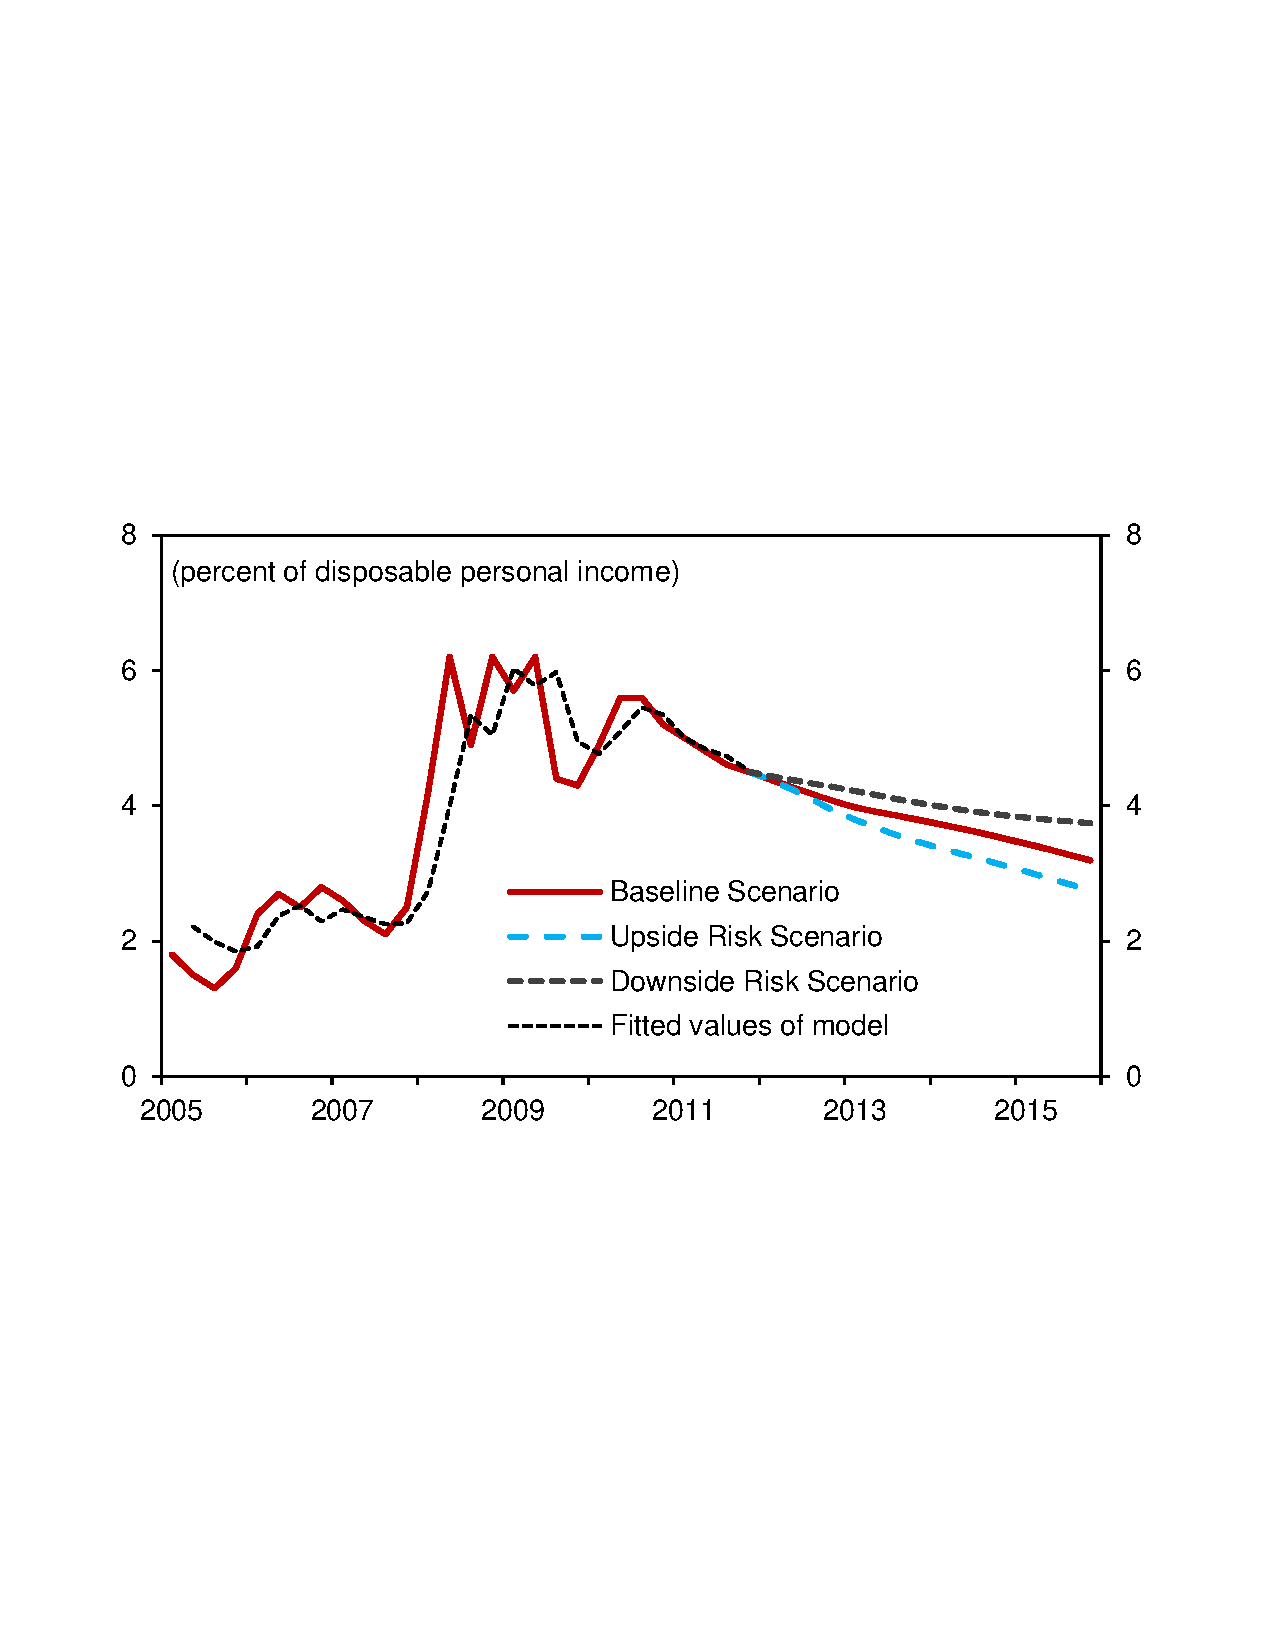
\includegraphics[width=4in]{\econtexRoot/Figures/fPSRforecast.pdf}

                                           Scenarios based on SPF and our judgement

                                         \end{frame}


                                         \begin{frame}
                                           \frametitle{\textbf{Conclusions}}

                                           \begin{itemize}
                                           \item All three effects present
                                           \item Easier borrowing largely explains secular decline $\sRat$
                                           \item Order of importance in Great Recession:
                                             \begin{enumerate}
                                             \item Wealth shock
                                             \item Labor income risk
                                             \item Credit tightening
                                               \ifPtn{
                                                 \begin{itemize}
                                                 \item $\Rightarrow$ if credit has big cyclical effect, comes thru $w$ and $\mho$
                                                 \end{itemize}}{}
                                               % \item Deleveraging/elevated saving rate likely to continue for a while
                                             \end{enumerate}
                                             \ifPtn{}{\item PSR to remain elevated}
                                           \end{itemize}

                                         \end{frame}


                                         \begin{frame}
                                           \frametitle{\textbf{References}}
                                           \tiny
                                           \bibliography{economics,cssUSSaving-Slides,cssUSSaving-Slides-Add}
                                           %
%\write18{if [ `kpsewhich economics.bib` != '' ]; then touch economics.bib    ; fi} # This should be done only for final versions AFTER bibexport has occurred and \jobname.bib is populated 
\write18{if [ ! -f \jobname.bib     ]; then touch \jobname.bib     ; fi}
\write18{if [ ! -f \jobname-Add.bib ]; then touch \jobname-Add.bib ; fi}

 
\bibliography{economics,\jobname,\jobname-Add}

                                         \end{frame}


                                         \begin{frame}
                                           \Large\remph{Background Slides}
                                         \end{frame}


                                         \begin{frame}\frametitle{\textbf{Alternative Measures of Credit Availability}}
                                           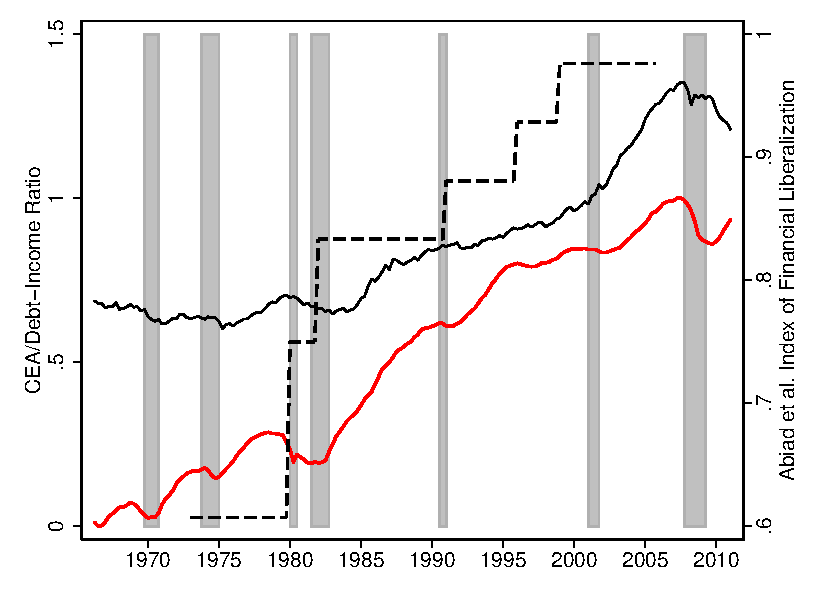
\includegraphics[width=4in]{\econtexRoot/Figures/fCreditAvailability_compare.pdf}
                                         \end{frame}


                                         \begin{frame}\frametitle{\textbf{Assumptions/Scenarios for Out-of-Sample Forecasts}}
                                           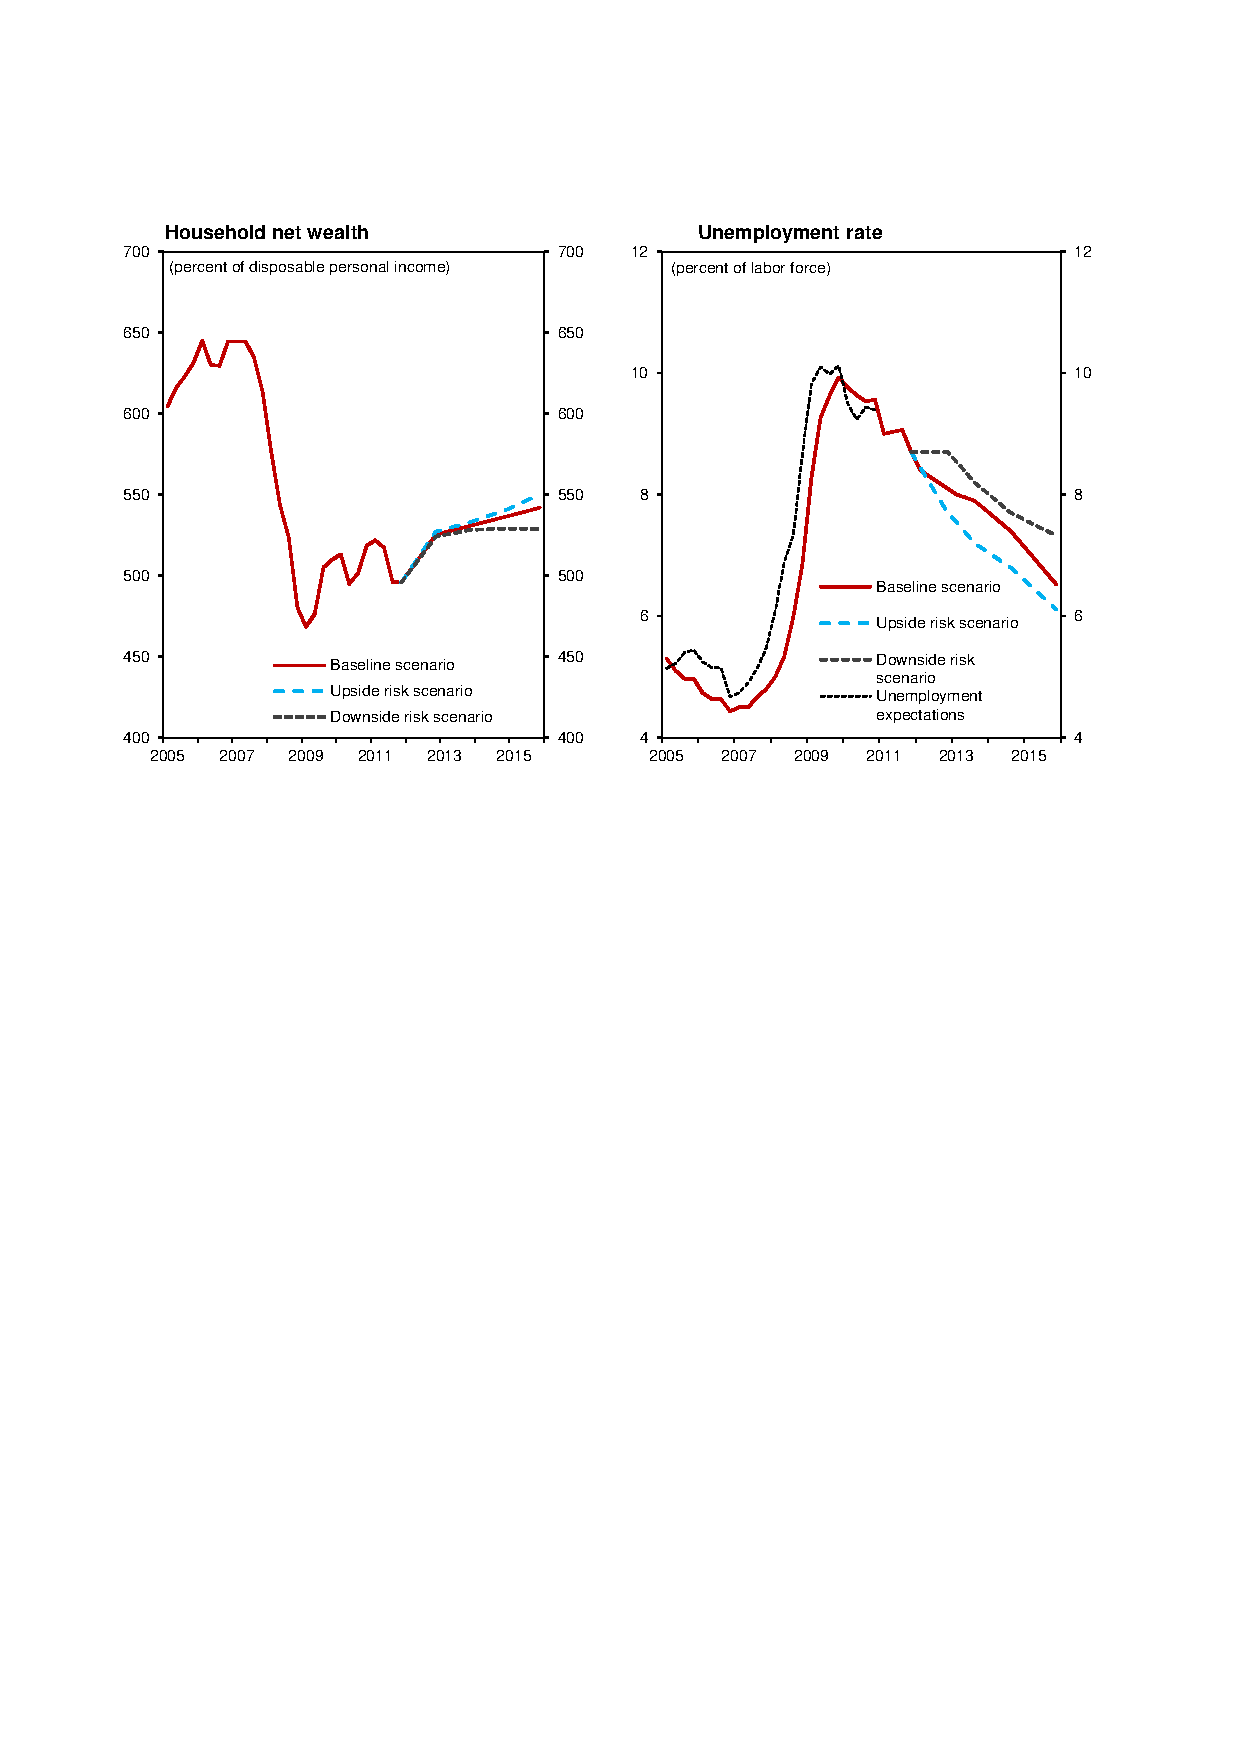
\includegraphics[width=4in]{\econtexRoot/Figures/fPSRforecastScenarios_1.pdf}
                                         \end{frame}


                                         \begin{frame}\frametitle{\textbf{Assumptions/Scenarios for Out-of-Sample Forecasts}}
                                           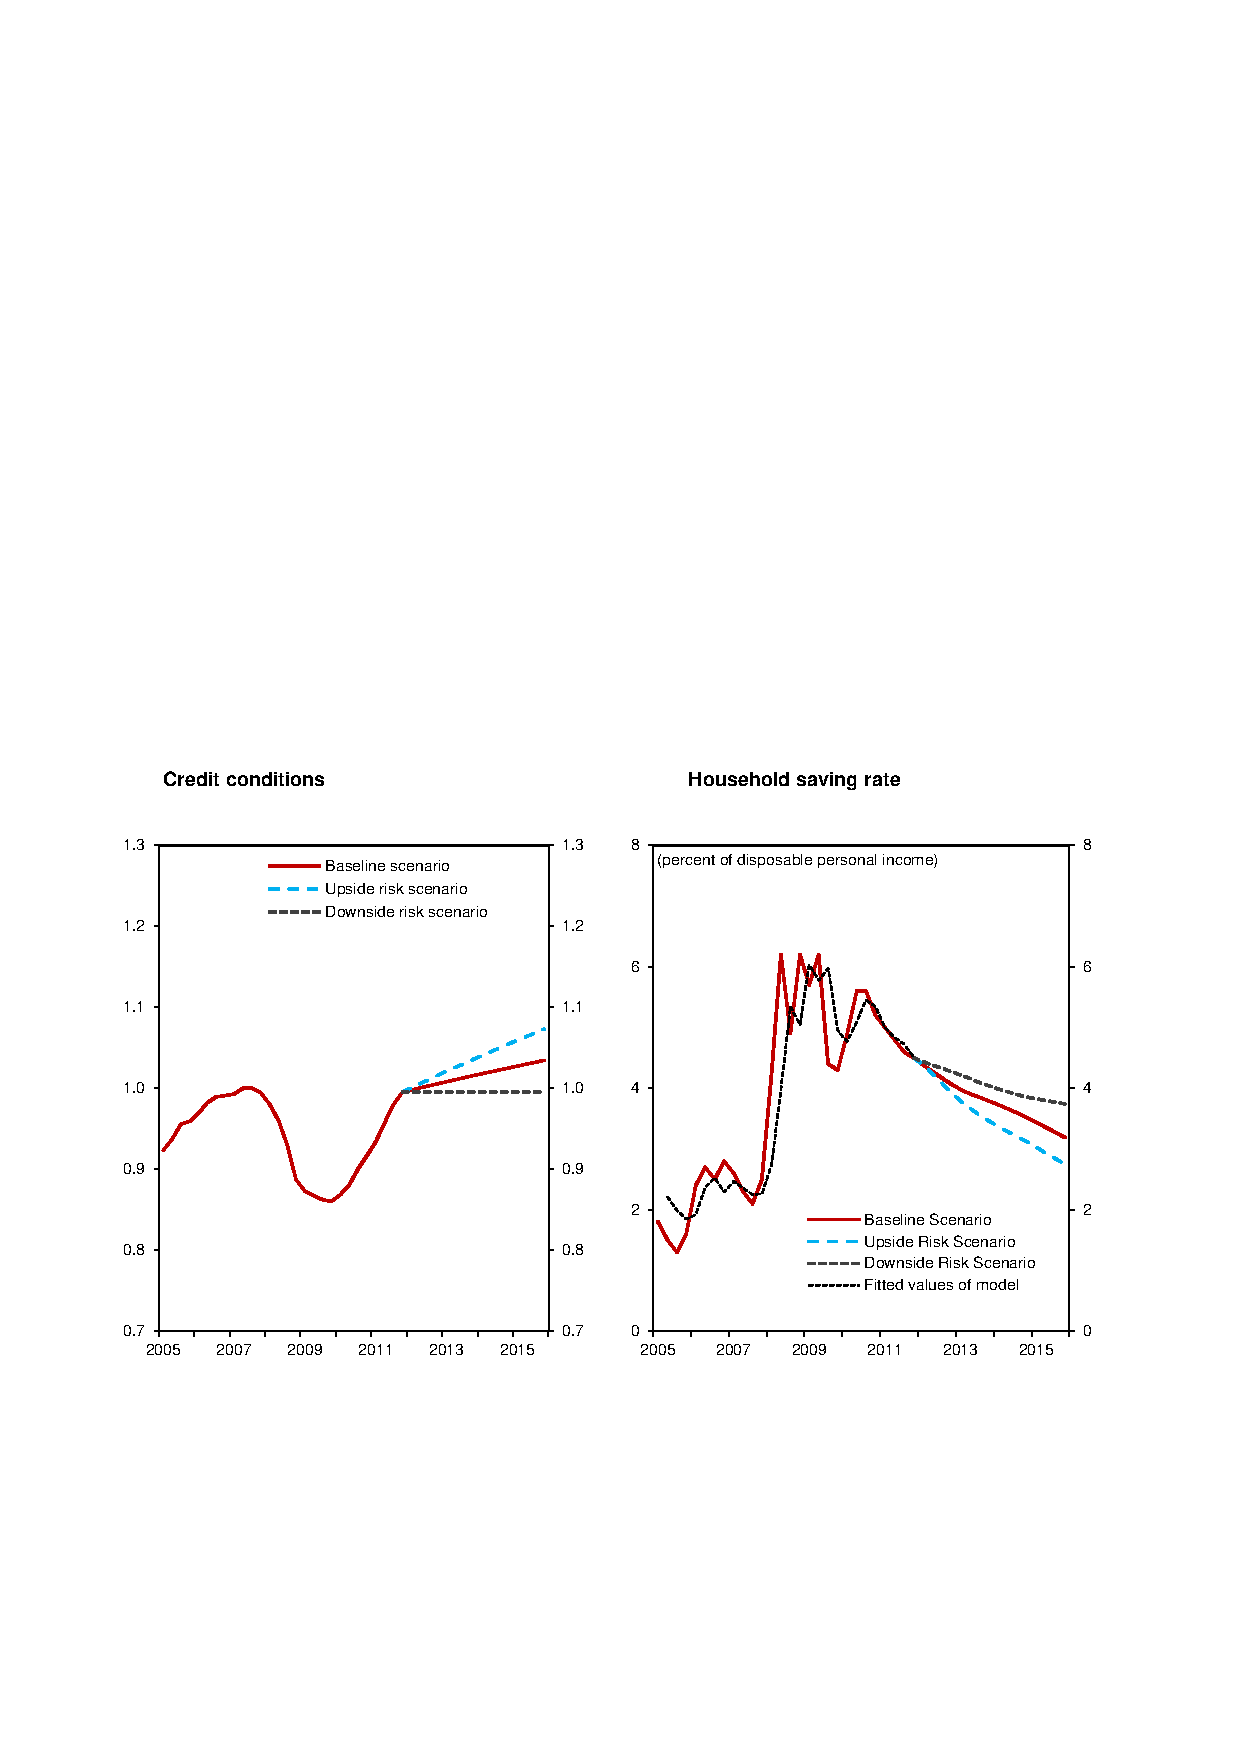
\includegraphics[width=4in]{\econtexRoot/Figures/fPSRforecastScenarios_2.pdf}
                                         \end{frame}

                                         \begin{frame}\frametitle{\textbf{Actual and Target Wealth}}
                                           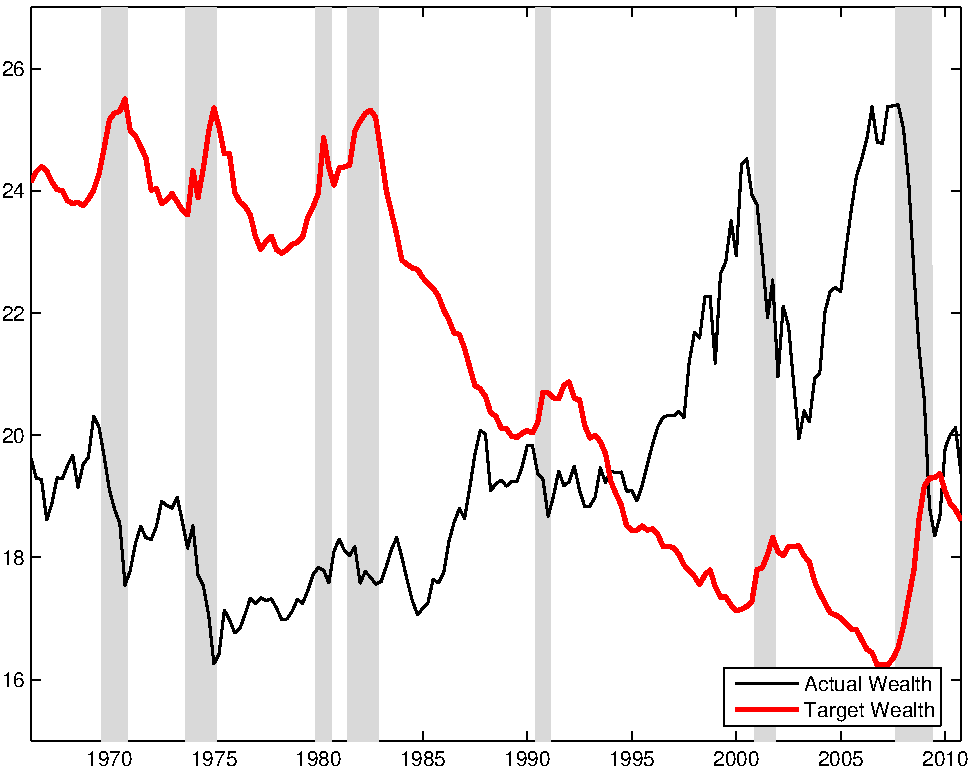
\includegraphics[width=4in]{\econtexRoot/Figures/fWealthTarget.pdf}
                                         \end{frame}


                                           \begin{frame}
    \frametitle{\textbf{Household Wealth 2007--  $\boldsymbol{\downarrow}$ by 150\% of Income}}

    \begin{figure}
      % \begin{center}
      %   \vspace*{-4mm}
      %   \hspace*{-1.0cm}
      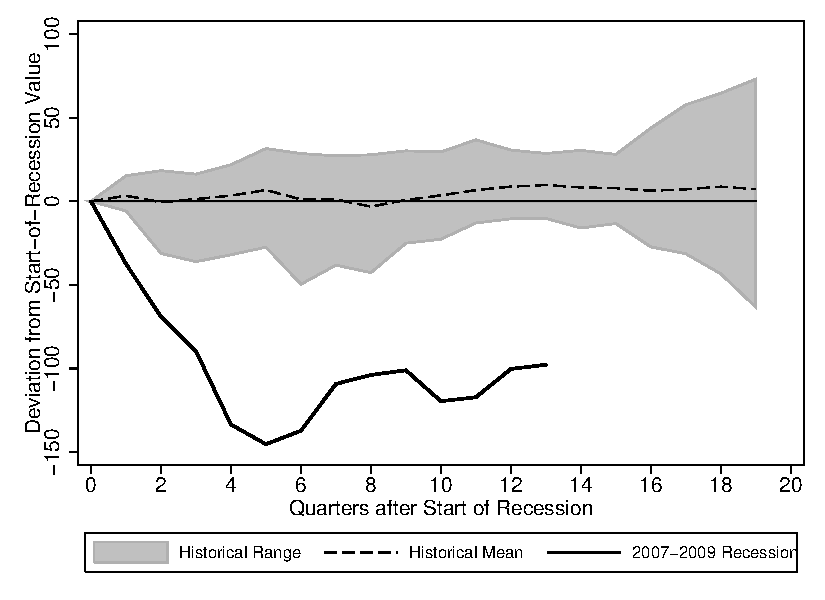
\includegraphics[height=3in,width=4.5in]{\econtexRoot/Figures/fWealth.pdf}
      % \end{center}
    \end{figure}
  \end{frame}

                                           \begin{frame}
    \frametitle{\textbf{Sustained Expectations of \underline{Rising} Unemp Risk}}
    Thomson Reuters/University of Michigan $\Ex_{t}(u_{t+4}-u_{t})$

    \begin{figure}
      % \begin{center}
      %   \vspace*{-4mm}
      %   \hspace*{-1.0cm}
      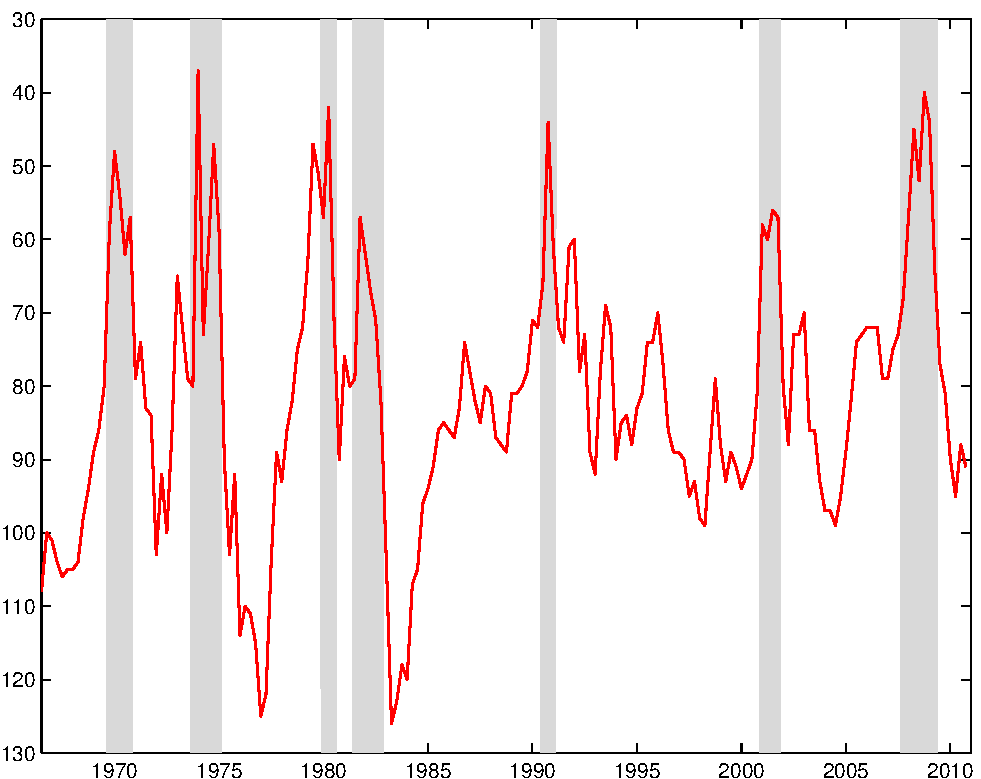
\includegraphics[height=2.8in,width=4.5in]{\econtexRoot/Figures/fUExp.pdf}
      % \end{center}
    \end{figure}
  \end{frame}

                                           \begin{frame}
    \frametitle{\textbf{Tighter  HH Credit Supply (Based on Muellbauer)}}

    \begin{figure}
      % \begin{center}
      %   \vspace*{-4mm}
      %   \hspace*{-1.0cm}
      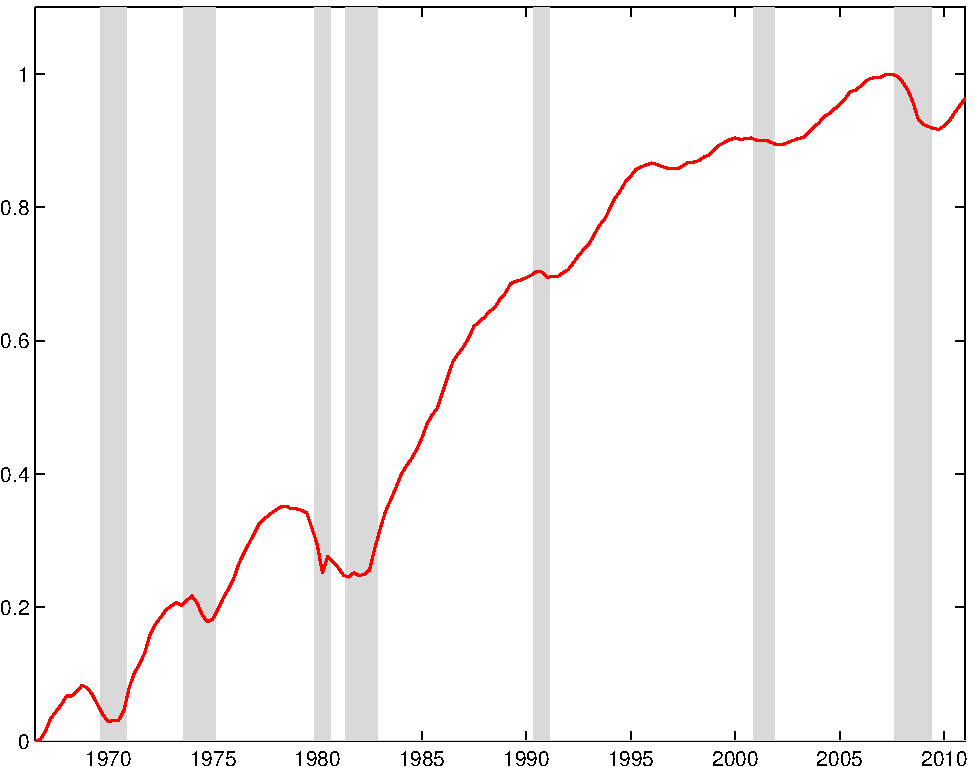
\includegraphics[height=3in,width=4.5in]{\econtexRoot/Figures/fCredit.pdf}
      % \end{center}
    \end{figure}
  \end{frame}

                                         \input \econtexRoot/Slides/PtnSlidesMovedToEnd-ConsFunc.tex
                                         \input \econtexRoot/Slides/PtnSlidesMovedToEnd-Overshooting.tex
                                         \input \econtexRoot/Slides/PtnSlidesMovedToEnd-ReducedForm.tex

                                       \end{document}
